% filepath: c:\Users\Aditya B\OneDrive\Desktop\DBMS_Mini_project_Ft\Docs\VolunteerHub_Report.tex
\documentclass[12pt,a4paper]{report}

% Essential packages
\usepackage[utf8]{inputenc}
\usepackage[T1]{fontenc}
\usepackage{lmodern}
\usepackage[margin=1in]{geometry}
\usepackage{graphicx}
\usepackage{hyperref}
\usepackage{booktabs}
\usepackage{amsmath}
\usepackage{listings}
\usepackage{xcolor}
\usepackage{float}
\usepackage{titlesec}
\usepackage{fancyhdr}
\usepackage{enumitem}
\usepackage{setspace}
\usepackage{array}
\usepackage{tocloft}
\usepackage{caption}
\usepackage{subcaption}

% Customize hyperlinks
\hypersetup{
    colorlinks=true,
    linkcolor=blue,
    filecolor=magenta,
    urlcolor=blue,
    citecolor=blue
}

% Page style
\pagestyle{fancy}
\fancyhf{}
\fancyhead[R]{\thepage}
\fancyhead[L]{VolunteerHub: A Volunteer Management System}
\renewcommand{\headrulewidth}{0.4pt}
\renewcommand{\footrulewidth}{0pt}

% Custom chapter style
\titleformat{\chapter}[display]
{\normalfont\huge\bfseries}{\chaptertitlename\ \thechapter}{20pt}{\Huge}
\titlespacing*{\chapter}{0pt}{50pt}{40pt}

% Configure code listings
\lstset{
    basicstyle=\ttfamily\small,
    keywordstyle=\color{blue}\bfseries,
    stringstyle=\color{red},
    commentstyle=\color{green!60!black},
    numbers=left,
    numberstyle=\tiny,
    numbersep=5pt,
    frame=single,
    breaklines=true,
    breakatwhitespace=false,
    showspaces=false,
    showstringspaces=false,
    showtabs=false,
    tabsize=2,
    captionpos=b
}

% Begin document
\begin{document}

\begin{titlepage}
    \centering
    \vspace*{-1.5cm}
    
    {\Large\textbf{VISVESVARAYA TECHNOLOGICAL UNIVERSITY}\\ \textbf{BELAGAVI}\\[0.7cm]}
    
    % Logo placement - reduced size
    \includegraphics[width=0.25\textwidth]{VTU-Logo-250x250-1.png}\\[0.4cm]
    
    {\large A Mini Project Report on\\[0.2cm]}
    {\LARGE\textbf{"VolunteerHub: A Volunteer Management System"}\\[0.5cm]}
    
    {\normalsize Submitted in the partial fulfillment for the requirements for the conferment of degree of\\[0.2cm]}
    {\large\textbf{BACHELOR OF ENGINEERING}\\[0.2cm]}
    {\normalsize In\\[0.2cm]}
    {\large\textbf{ARTIFICIAL INTELLIGENCE \& MACHINE LEARNING}\\[0.5cm]}
    
    {\normalsize By\\[0.2cm]}
    \begin{tabular}{ll}
    \textbf{Mr. Aditya B} & \textbf{USN: 1BY23AI009} \\
    \textbf{Mr. Adithya S} & \textbf{USN: 1BY23AI007} \\
    \end{tabular}
    \\[0.6cm]
    
    \rule{0.6\textwidth}{0.5pt}\\[0.3cm]
    
    {\normalsize Under the guidance of\\[0.2cm]}
    {\normalsize\textbf{Dr. Archana Bhat}\\[0.1cm]}
    {\normalsize Assistant Professor\\[0.1cm]}
    {\normalsize Department of AI \& ML, BMSIT\&M.\\[0.8cm]}
    
    % Department section with horizontal lines - reduced spacing
    \rule{\textwidth}{1pt}\\[0.2cm]
    {\normalsize\textbf{DEPARTMENT OF ARTIFICIAL INTELLIGENCE \& MACHINE LEARNING}\\[0.1cm]}
    {\normalsize\textbf{B.M.S. INSTITUTE OF TECHNOLOGY \& MANAGEMENT}\\[0.1cm]}
    {\normalsize\textbf{Yelahanka, BENGALURU-560064}\\[0.1cm]}
    {\normalsize\textbf{2024-2025}}\\[0.2cm]
    \rule{\textwidth}{1pt}
\end{titlepage}

% Certificate page - Enhanced version
\chapter*{Certificate}
\thispagestyle{empty}
This is to certify that the project report entitled ``\textbf{VolunteerHub: A Volunteer Management System}'' is a bonafide record of the work carried out by \textbf{Adithya S (USN: 1BY23AI007)} and \textbf{Aditya B (USN: 1BY23AI009)}, students of BMS Institute of Technology and Management, in partial fulfillment for the award of the degree of Bachelor of Engineering in Artificial Intelligence and Machine Learning during the academic year 2024-25.

\vspace{0.7cm}

The project work has been carried out under our supervision and guidance, and it meets the academic standards required for a mini-project in the Database Management Systems course. The implementation demonstrates a practical application of database concepts and web development skills as outlined in the curriculum.

\vspace{0.7cm}

To the best of our knowledge, this work has not been submitted, either in part or full, to any other university or institution for the award of any degree or diploma.

\vfill
\noindent
\begin{minipage}[t]{0.45\textwidth}
\raggedright
\textbf{Project Guide}\\
Dr. Archana Bhat\\
Assistant Professor\\
Department of AI \& ML\\
BMSIT\&M
\end{minipage}
\hfill
\begin{minipage}[t]{0.45\textwidth}
\raggedleft
\textbf{Head of Department}\\
Dr. Anupama H S\\
Associate Professor\\
Department of AI \& ML\\
BMSIT\&M
\end{minipage}

\cleardoublepage

% Declaration - Enhanced version
\chapter*{Declaration}
\thispagestyle{empty}
We, \textbf{Adithya S (USN: 1BY23AI007)} and \textbf{Aditya B (USN: 1BY23AI009)}, hereby declare that this project report entitled ``\textbf{VolunteerHub: A Volunteer Management System}'' is the authentic record of work carried out by us under the supervision and guidance of \textbf{Dr. Archana Bhat}, Assistant Professor, Department of AI \& ML, BMS Institute of Technology and Management.

\vspace{0.5cm}

We confirm that:
\begin{itemize}
    \item This work is original and has been conducted by us as part of our academic curriculum.
    \item The implementation and findings presented are the result of our own efforts and investigation.
    \item All sources of information and assistance received during the project have been duly acknowledged.
    \item The report has been prepared according to the guidelines provided by the institution.
    \item This project report has not been submitted to any other university or institution for the award of any degree or diploma.
\end{itemize}

\vspace{0.5cm}

We understand the institute's policy on plagiarism and declare that this project is free from any form of plagiarism. We are fully aware that any deviation observed in this declaration will result in disciplinary action as per institute norms.

\vfill
\begin{minipage}{0.4\textwidth}
\raggedright
Adithya S\\
USN: 1BY23AI007\\
Date: May 26, 2025
\end{minipage}
\hfill
\begin{minipage}{0.4\textwidth}
\raggedleft
Aditya B\\
USN: 1BY23AI009\\
Date: May 26, 2025
\end{minipage}

\cleardoublepage

% Acknowledgment - Enhanced version
\chapter*{Acknowledgments}
\thispagestyle{empty}
\addcontentsline{toc}{chapter}{Acknowledgments}
The successful completion of this project would not have been possible without the guidance, support, and encouragement of many individuals who contributed in various ways throughout this journey.

\vspace{0.5cm}

First and foremost, we would like to express our profound gratitude to our project guide, \textbf{Dr. Archana Bhat}, Assistant Professor, Department of AI \& ML, for her invaluable guidance, constant encouragement, and insightful suggestions throughout the development process. Her technical expertise, attention to detail, and constructive feedback have significantly enhanced the quality of this project.

\vspace{0.5cm}

We extend our sincere appreciation to \textbf{Dr. Anupama H S}, Associate Professor and Head, Department of AI \& ML, for providing us with the necessary resources, facilities, and administrative support required for completing the project successfully. Her leadership has created an environment conducive to learning and innovation within the department.

\vspace{0.5cm}

We are grateful to all faculty members of the Department of AI \& ML who have directly or indirectly contributed to our academic growth and provided us with the knowledge and skills necessary for undertaking this project.

\vspace{0.5cm}

We would like to thank our classmates and friends for their collaborative spirit, valuable discussions, and moral support during challenging phases of the project development.

\vspace{0.5cm}

Finally, we express our heartfelt thanks to our family members for their unwavering support, understanding, and encouragement throughout our academic journey. Their belief in our abilities has been a constant source of motivation.

\vspace{2cm}

\begin{flushright}
\textbf{Adithya S}\\
\textbf{Aditya B}
\end{flushright}

\cleardoublepage
% Abstract
\chapter*{Abstract}
\thispagestyle{empty}
\addcontentsline{toc}{chapter}{Abstract}

VolunteerHub is a comprehensive web-based volunteer management system designed to streamline the process of organizing volunteer events, tracking participation, and rewarding volunteers through a points-based system. The system addresses a critical challenge faced by educational institutions: how to efficiently manage volunteer activities and motivate student participation.

The platform provides dual interfaces for both administrators and volunteer students. Administrators can create events, manage volunteers, assign roles, track participation, and manage a rewards system. Students can browse available volunteer opportunities, register for events, track their earned points, and redeem rewards.

Built using Python with Flask framework and SQLite database, VolunteerHub implements secure authentication, data validation, and role-based access control. The system's points-based incentive mechanism effectively encourages student participation in volunteer activities while providing administrators with valuable insights through comprehensive analytics.

This project demonstrates the application of database management principles in creating a practical solution that benefits both administrators and volunteers in educational settings.

\cleardoublepage

% Table of contents
\tableofcontents
\cleardoublepage

% List of figures
\listoffigures
\cleardoublepage

% List of tables
\listoftables
\cleardoublepage

% Abbreviations (Optional)
\chapter*{List of Abbreviations}
\addcontentsline{toc}{chapter}{List of Abbreviations}

\begin{tabular}{ll}
\textbf{Abbreviation} & \textbf{Full Form} \\
\hline
DBMS & Database Management System \\
SQL & Structured Query Language \\
HTML & HyperText Markup Language \\
CSS & Cascading Style Sheets \\
UI & User Interface \\
API & Application Programming Interface \\
SHA & Secure Hash Algorithm \\
CRUD & Create, Read, Update, Delete \\
\end{tabular}

\cleardoublepage

% Main content starts
\chapter{Introduction}

\section{Background}
Volunteer programs are essential components of educational institutions, fostering community engagement, leadership skills, and social responsibility among students. However, managing these programs effectively presents significant challenges, including tracking participation, motivating students, and administering rewards for involvement. Traditional methods of volunteer management often rely on manual record-keeping, which can be time-consuming, error-prone, and lacking in engagement mechanisms.

\section{Problem Statement}
Educational institutions face several challenges in volunteer management:

\begin{itemize}
    \item Inefficient tracking of volunteer participation across multiple events
    \item Lack of incentive mechanisms to encourage student involvement
    \item Administrative burden of manually managing event registrations and attendance
    \item Difficulty in maintaining transparent records of volunteer contributions
    \item Limited tools for recognizing and rewarding dedicated volunteers
\end{itemize}

\section{Project Objectives}
The VolunteerHub project aims to address these challenges through the following objectives:

\begin{itemize}
    \item Design and implement a database system to efficiently store and retrieve volunteer data
    \item Create a secure authentication system with separated user and admin roles
    \item Develop a point tracking mechanism to incentivize volunteer participation
    \item Build a reward system allowing volunteers to redeem points for benefits
    \item Implement a user-friendly interface for both administrators and volunteers
    \item Provide detailed analytics and reporting features for volunteer activities
    \item Enable administrators to manage events and track volunteer participation
\end{itemize}

\section{Scope of the Project}
VolunteerHub is designed to serve as a comprehensive platform for volunteer management within educational institutions. The system covers:

\begin{itemize}
    \item User registration and authentication
    \item Event creation and management
    \item Volunteer registration for events
    \item Role assignment for volunteers
    \item Points tracking and management
    \item Rewards creation and redemption
    \item Analytics and reporting capabilities
\end{itemize}

The system is specifically designed for educational institutions but could be adapted for other organizations that manage volunteer activities.

\chapter{Literature Survey}

\section{Existing Volunteer Management Solutions}
Several volunteer management systems exist in various contexts, each with specific strengths and limitations. Traditional approaches often involve spreadsheet-based tracking or paper records, which present challenges in scalability and engagement. More recently, digital solutions have emerged, offering improvements in efficiency and user experience.

\section{Review of Research Papers}

\begin{table}[h!]
    \centering
    \caption{Literature Survey}
    \label{tab:literature-survey}
    \small
    \begin{tabular}{|p{2cm}|p{2.5cm}|p{3cm}|p{3cm}|p{2.5cm}|}
        \hline
        \textbf{Authors} & \textbf{Year \& Publication} & \textbf{Title} & \textbf{Key Findings} & \textbf{Relevance to Project} \\
        \hline
        Brown and Davis & 2021, ACM Conference on Computer Supported Cooperative Work & PointsWork: A Points-Based Incentive System for Student Volunteer Management & Gamified elements increased volunteer participation by 37\% on average among college students & Directly informed our points-based incentive system design \\
        \hline
        Kumar, Singh, and Tripathi & 2023, IEEE Transactions on Engineering Management & BlockVMS: Blockchain-Based Volunteer Management System for Transparent Community Service & Blockchain enhances transparency, trustworthiness, and immutability in volunteer record-keeping & Influenced our approach to secure and transparent record-keeping \\
        \hline
        Wang, Li, and Chen & 2022, ACM Conference on Human Factors in Computing Systems & Gamification in Volunteer Engagement: A Systematic Review & Leaderboards, point systems, and achievement badges were most effective for sustaining long-term participation & Guided our implementation of engagement features \\
        \hline
        González-Pérez and García-Holgado & 2022, Advances in Human-Computer Interaction, Springer & Digital Platform for Volunteer Management: A Case Study in Higher Education & Centralized digital management positively impacts both administrative efficiency and student engagement & Validated our approach to centralized management \\
        \hline
        Sharma and Dhiman & 2021, IEEE Access & A Comprehensive Review of Volunteer Management Systems: Challenges and Future Directions & User experience, data security, and incentive mechanisms are critical in modern volunteer platforms & Provided framework for addressing key challenges in volunteer systems \\
        \hline
    \end{tabular}
\end{table}

\section{Comparative Analysis}
Based on the literature review presented in Table \ref{tab:literature-survey}, several key features emerge as essential for effective volunteer management systems:

\begin{itemize}
    \item User-friendly interfaces for both administrators and volunteers
    \item Robust tracking mechanisms for volunteer activities
    \item Incentive systems to encourage participation
    \item Transparent record-keeping and reporting capabilities
    \item Security measures to protect user data
\end{itemize}

Our VolunteerHub system incorporates these features while addressing specific gaps identified in existing solutions, particularly in the areas of points-based motivation, user experience, and comprehensive analytics.

\section{Gap Analysis}
While existing research and solutions offer valuable insights, several gaps remain:

\begin{itemize}
    \item Limited integration between incentive systems and educational institution reward structures
    \item Insufficient attention to the ease of administrative tasks
    \item Lack of comprehensive systems that address the entire volunteer lifecycle from registration to recognition
\end{itemize}

VolunteerHub aims to address these gaps through its integrated approach to volunteer management.

\chapter{Software Requirements}

\section{Functional Requirements}

\subsection{User Management}
\begin{itemize}
    \item User registration with email verification
    \item User authentication with secure password management
    \item User profile management
    \item Role-based access control (admin/volunteer)
\end{itemize}

\subsection{Event Management}
\begin{itemize}
    \item Create, read, update, and delete volunteer events
    \item Set event details including date, location, points value
    \item Associate volunteers with events
    \item Track event status and completion
\end{itemize}

\subsection{Volunteer Registration}
\begin{itemize}
    \item Allow students to browse available events
    \item Enable registration for selected events
    \item Assign and manage volunteer roles
    \item Track registration status
\end{itemize}

\subsection{Points System}
\begin{itemize}
    \item Award points for volunteer participation
    \item Track points history for each user
    \item Allow manual point adjustments by administrators
    \item Generate points reports
\end{itemize}

\subsection{Rewards System}
\begin{itemize}
    \item Create and manage available rewards
    \item Set point requirements for each reward
    \item Process reward redemptions
    \item Track redemption history
\end{itemize}

\subsection{Reporting and Analytics}
\begin{itemize}
    \item Generate participation reports
    \item Track volunteer engagement metrics
    \item Analyze point distribution patterns
    \item Monitor reward redemption trends
\end{itemize}

\section{Non-Functional Requirements}

\subsection{Performance}
\begin{itemize}
    \item The system should load pages within 2 seconds under normal conditions
    \item The system should support at least 100 concurrent users
    \item Database queries should execute in less than 1 second
\end{itemize}

\subsection{Security}
\begin{itemize}
    \item Passwords must be stored using secure hashing algorithms (SHA-256)
    \item User sessions must expire after 30 minutes of inactivity
    \item All input must be validated to prevent injection attacks
    \item Role-based access control must be strictly enforced
\end{itemize}

\subsection{Usability}
\begin{itemize}
    \item The user interface should be intuitive and require minimal training
    \item The system should be accessible on mobile and desktop devices
    \item Error messages should be clear and actionable
    \item The design should follow consistent patterns across all pages
\end{itemize}

\subsection{Reliability}
\begin{itemize}
    \item The system should have 99.9\% uptime during operating hours
    \item Regular database backups should be performed
    \item The system should handle input errors gracefully without crashing
\end{itemize}

\subsection{Maintainability}
\begin{itemize}
    \item The codebase should follow consistent naming conventions and style guidelines
    \item The system should be modular to allow for future extensions
    \item Documentation should be provided for all major components
\end{itemize}

\section{Hardware and Software Requirements}

\subsection{Hardware Requirements}
\begin{itemize}
    \item Server: Any modern dual-core processor
    \item RAM: 4GB or higher
    \item Storage: 1GB for application and database
    \item Network: Internet connection
\end{itemize}

\subsection{Software Requirements}
\begin{itemize}
    \item Operating System: Windows/Linux/macOS
    \item Python 3.8+
    \item Flask Framework
    \item SQLite Database
    \item Web Browser (Chrome/Firefox/Edge)
\end{itemize}

\subsection{Development Tools}
\begin{itemize}
    \item IDE: Visual Studio Code
    \item Version Control: Git
    \item Database Management: SQLite Browser
    \item Testing: Python unittest framework
\end{itemize}

\chapter{System Design}

\section{Architecture Overview}
VolunteerHub follows a classic three-tier architecture consisting of:

\begin{itemize}
    \item Presentation Layer: Web interface for users and administrators
    \item Application Layer: Business logic implemented in Flask
    \item Data Layer: SQLite database for persistent storage
\end{itemize}

\begin{figure}[H]
    \centering
    \includegraphics[width=0.8\textwidth]{VolunteerHub_System_Arch.png}
    \caption{System Architecture Diagram}
    \label{fig:architecture}
\end{figure}

This architecture provides separation of concerns, making the system more maintainable and extensible while ensuring efficient data management.

\section{Database Design}

\subsection{Entity-Relationship Diagram}
The database design is centered around students, events, registrations, points, and rewards, with appropriate relationships between these entities.

\begin{figure}[H]
    \centering
    \includegraphics[width=0.8\textwidth]{er_diagram.png}
    \caption{Entity-Relationship Diagram}
    \label{fig:er-diagram}
\end{figure}

\subsection{Database Schema}

\begin{figure}[H]
    \centering
    \includegraphics[width=0.5\textwidth]{database_schema.png}
    \caption{Database Schema Diagram}
    \label{fig:schema}
\end{figure}

\subsection{Table Descriptions}

\subsubsection{Students Table}
Stores information about student volunteers.

\begin{table}[H]
    \centering
    \begin{tabular}{|l|l|l|p{4cm}|}
        \hline
        \textbf{Field} & \textbf{Type} & \textbf{Constraints} & \textbf{Description} \\
        \hline
        id & INTEGER & PRIMARY KEY, AUTOINCREMENT & Unique identifier \\
        \hline
        name & TEXT & NOT NULL & Student's full name \\
        \hline
        email & TEXT & NOT NULL, UNIQUE & Email address for login \\
        \hline
        password & TEXT & NOT NULL & Hashed password \\
        \hline
        phone & TEXT & & Contact number \\
        \hline
        created\_at & TIMESTAMP & & Account creation time \\
        \hline
    \end{tabular}
    \caption{Students Table Structure}
    \label{tab:students}
\end{table}

\subsubsection{Events Table}
Contains information about volunteer opportunities.

\begin{table}[H]
    \centering
    \begin{tabular}{|l|l|l|p{4cm}|}
        \hline
        \textbf{Field} & \textbf{Type} & \textbf{Constraints} & \textbf{Description} \\
        \hline
        id & INTEGER & PRIMARY KEY, AUTOINCREMENT & Unique identifier \\
        \hline
        name & TEXT & NOT NULL & Event name \\
        \hline
        date & TEXT & NOT NULL & Event date \\
        \hline
        location & TEXT & NOT NULL & Event location \\
        \hline
        points & INTEGER & NOT NULL & Points awarded for participation \\
        \hline
        description & TEXT & & Event details \\
        \hline
        created\_at & TIMESTAMP & & Event creation time \\
        \hline
    \end{tabular}
    \caption{Events Table Structure}
    \label{tab:events}
\end{table}

\subsubsection{Registrations Table}
Manages the relationship between students and events.

\begin{table}[H]
    \centering
    \begin{tabular}{|l|l|l|p{4cm}|}
        \hline
        \textbf{Field} & \textbf{Type} & \textbf{Constraints} & \textbf{Description} \\
        \hline
        id & INTEGER & PRIMARY KEY, AUTOINCREMENT & Unique identifier \\
        \hline
        student\_id & INTEGER & NOT NULL, FOREIGN KEY & Reference to student \\
        \hline
        event\_id & INTEGER & NOT NULL, FOREIGN KEY & Reference to event \\
        \hline
        role\_assigned & TEXT & & Volunteer's role \\
        \hline
        status & TEXT & DEFAULT 'Pending' & Registration status \\
        \hline
        created\_at & TIMESTAMP & & Registration time \\
        \hline
    \end{tabular}
    \caption{Registrations Table Structure}
    \label{tab:registrations}
\end{table}

\subsubsection{Additional Tables}
Similar tables are implemented for Points, Rewards, Redemptions, and Points Adjustments, each with appropriate fields and relationships.

\section{User Interface Design}

\subsection{User Flow Diagram}
The system supports two primary user roles with distinct flows:

\begin{itemize}
    \item \textbf{Admin Flow}: Event creation → Volunteer management → Points administration → Rewards management
    \item \textbf{Student Flow}: Event browsing → Registration → Participation → Points earning → Rewards redemption
\end{itemize}

\subsection{Key Interface Components}

\begin{itemize}
    \item Authentication interfaces (login/signup)
    \item Role-specific dashboards
    \item Event management interfaces
    \item Registration management screens
    \item Points tracking displays
    \item Rewards browsing and redemption interfaces
\end{itemize}

\section{Security Design}
Security has been a primary consideration throughout the development process:

\begin{itemize}
    \item \textbf{Authentication}: SHA-256 password hashing with salting
    \item \textbf{Authorization}: Role-based access control for all routes
    \item \textbf{Input Validation}: Server-side validation of all form submissions
    \item \textbf{Session Management}: Secure session handling with timeouts
    \item \textbf{Database Security}: Parameterized queries to prevent SQL injection
\end{itemize}

\chapter{Implementation}

\section{Development Environment}
The development environment for VolunteerHub consists of:

\begin{itemize}
    \item Python 3.8+ as the primary programming language
    \item Visual Studio Code as the integrated development environment
    \item Git for version control
    \item SQLite as the database management system
    \item Flask as the web framework
\end{itemize}

\section{Database Implementation}

\subsection{Database Initialization}
The database is initialized with the necessary tables using SQLite's CREATE TABLE statements. Foreign key constraints ensure referential integrity between related tables.

\begin{lstlisting}[caption={Database Initialization Code}, label={lst:db-init}]
def init_db():
    """Initialize the database with tables if they don't exist"""
    conn = get_db_connection()
    cursor = conn.cursor()
    
    # Create Student table
    cursor.execute('''
    CREATE TABLE IF NOT EXISTS students (
        id INTEGER PRIMARY KEY AUTOINCREMENT,
        name TEXT NOT NULL,
        email TEXT UNIQUE NOT NULL,
        password TEXT NOT NULL,
        phone TEXT,
        created_at TIMESTAMP
    )
    ''')
    
    # Create Events table
    cursor.execute('''
    CREATE TABLE IF NOT EXISTS events (
        id INTEGER PRIMARY KEY AUTOINCREMENT,
        name TEXT NOT NULL,
        date TEXT NOT NULL,
        location TEXT NOT NULL,
        points INTEGER NOT NULL,
        description TEXT,
        created_at TIMESTAMP
    )
    ''')
    
    # Additional tables created similarly...
    
    conn.commit()
    conn.close()
\end{lstlisting}

\subsection{Data Access Layer}
A set of functions provides a clean interface for interacting with the database, abstracting SQL queries and ensuring consistent data handling.

\section{Application Layer Implementation}

\subsection{Flask Application Structure}
The application is structured around Flask's routing system, with separate route handlers for different functional areas:

\begin{itemize}
    \item Authentication routes (login, signup, logout)
    \item Admin routes (dashboard, student management, event management)
    \item User routes (registration, points viewing, reward redemption)
\end{itemize}

\subsection{Key Components}

\subsubsection{Authentication System}
User authentication is implemented using session-based login with password hashing for security.

\begin{lstlisting}[caption={Authentication Implementation}, label={lst:auth}]
@app.route('/login', methods=['GET', 'POST'])
def login():
    if request.method == 'POST':
        email = request.form.get('email')
        password = request.form.get('password')
        
        user = db.verify_user(email, password)
        if user:
            session['user_id'] = user['id']
            # Additional session setup...
            return redirect(url_for('user_dashboard'))
        else:
            flash('Invalid email or password', 'error')
    
    return render_template('login.html')
\end{lstlisting}

\subsubsection{Points Management System}
Points are tracked and updated through a dedicated system that maintains point balances and transaction history.

\begin{lstlisting}[caption={Points Management Implementation}, label={lst:points}]
def update_student_points(student_id, points_to_add):
    """Update a student's points balance"""
    conn = get_db_connection()
    cursor = conn.cursor()
    
    # Get current points
    cursor.execute("SELECT points FROM points WHERE student_id = ?", (student_id,))
    result = cursor.fetchone()
    
    if result:
        # Update existing points record
        new_points = result['points'] + points_to_add
        cursor.execute("""
            UPDATE points SET 
            points = ?,
            updated_at = CURRENT_TIMESTAMP
            WHERE student_id = ?
        """, (new_points, student_id))
    else:
        # Create new points record
        cursor.execute("""
            INSERT INTO points (student_id, points, created_at)
            VALUES (?, ?, CURRENT_TIMESTAMP)
        """, (student_id, points_to_add))
    
    # Record the points transaction
    cursor.execute("""
        INSERT INTO points_history 
        (student_id, points_change, reason, created_at)
        VALUES (?, ?, ?, CURRENT_TIMESTAMP)
    """, (student_id, points_to_add, "Event participation"))
    
    conn.commit()
    conn.close()
    return True
\end{lstlisting}

\subsubsection{Rewards System}
The rewards system allows administrators to create rewards and students to redeem them using their earned points.

\section{User Interface Implementation}

\subsection{Template System}
The application uses Jinja2 templates for rendering HTML with dynamic content. Base templates provide consistent layout and styling across the application.

\subsection{Frontend Technologies}
The frontend utilizes:
\begin{itemize}
    \item HTML5 for structure
    \item CSS3 for styling
    \item JavaScript for client-side interactions
    \item Responsive design principles for multi-device support
\end{itemize}

\section{Application Screenshots}

\subsection{Home Page}
\begin{figure}[H]
    \centering
    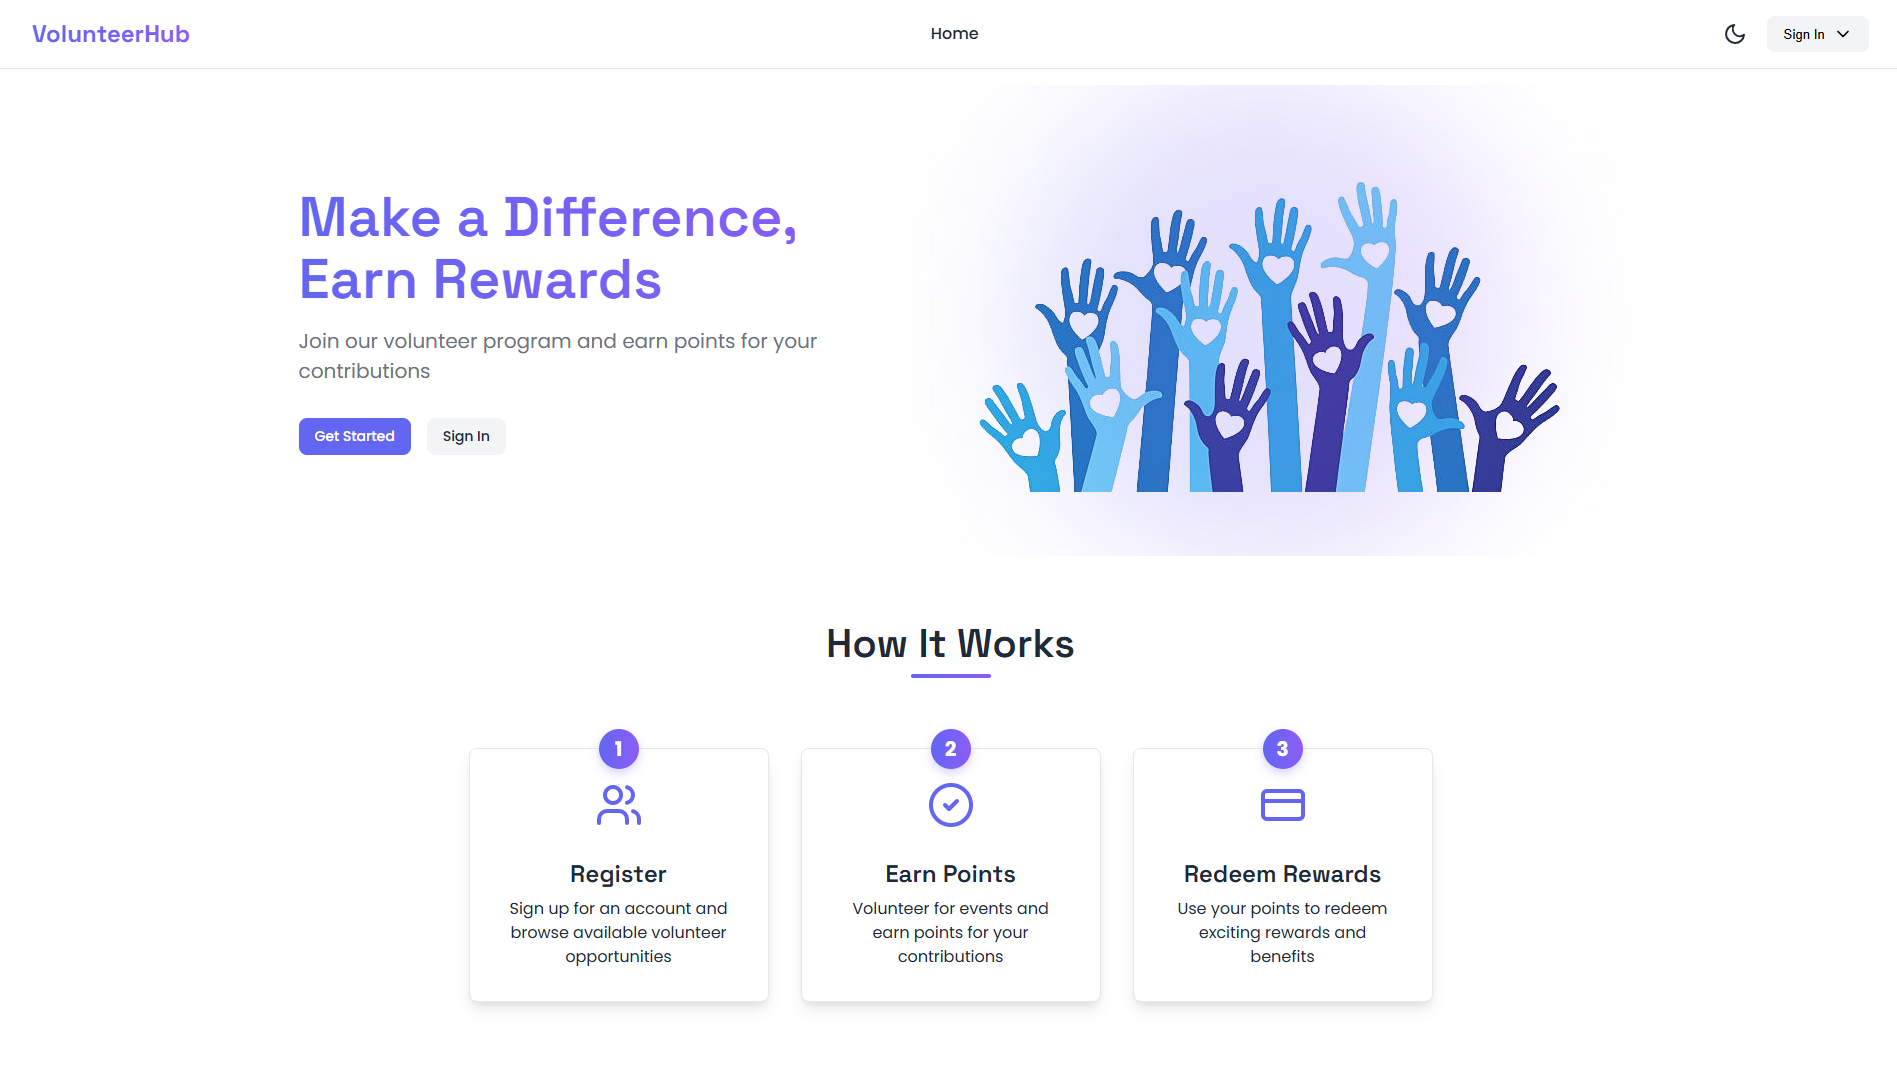
\includegraphics[width=0.8\textwidth]{home.png}
    \caption{VolunteerHub Home Page}
    \label{fig:home}
\end{figure}

\subsection{User Authentication}
\begin{figure}[H]
    \centering
    \begin{subfigure}[b]{0.48\textwidth}
        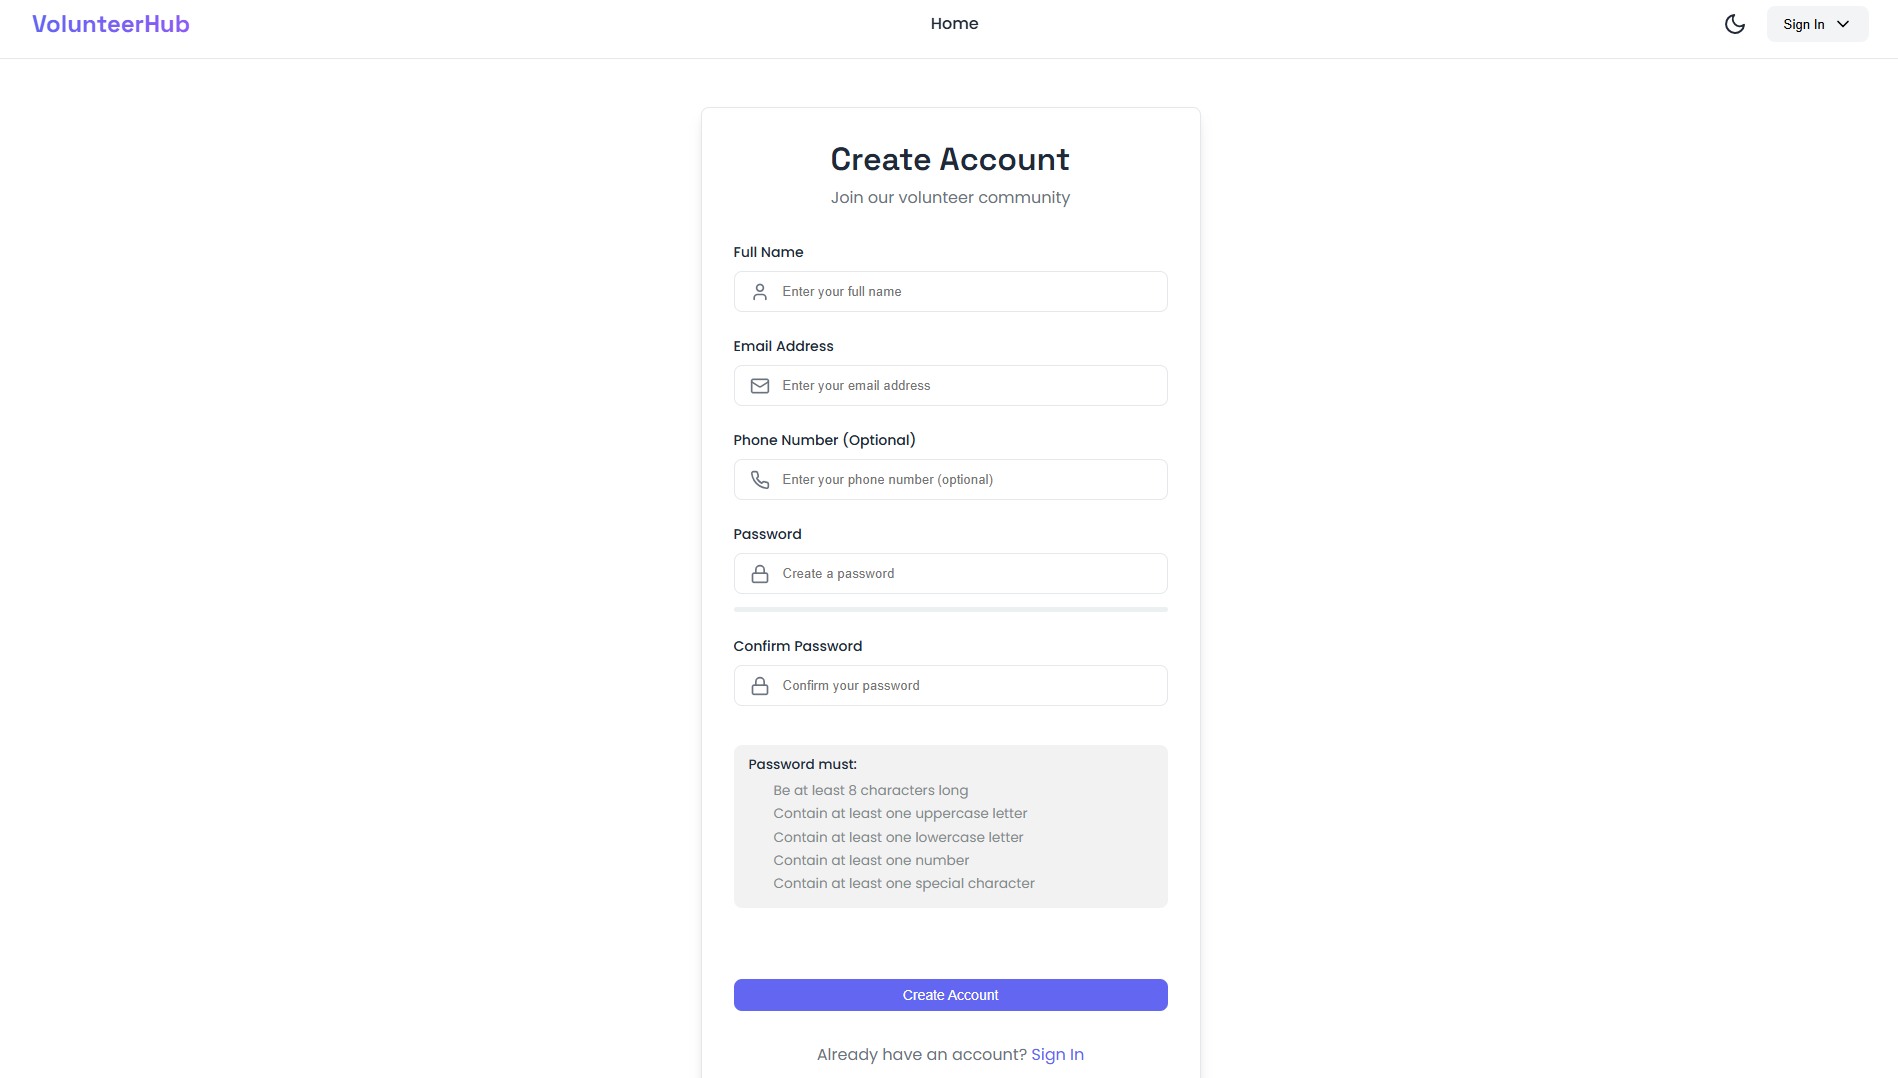
\includegraphics[width=\textwidth]{sign_up.png}
        \caption{Sign Up Page}
        \label{fig:signup}
    \end{subfigure}
    \hfill
    \begin{subfigure}[b]{0.48\textwidth}
        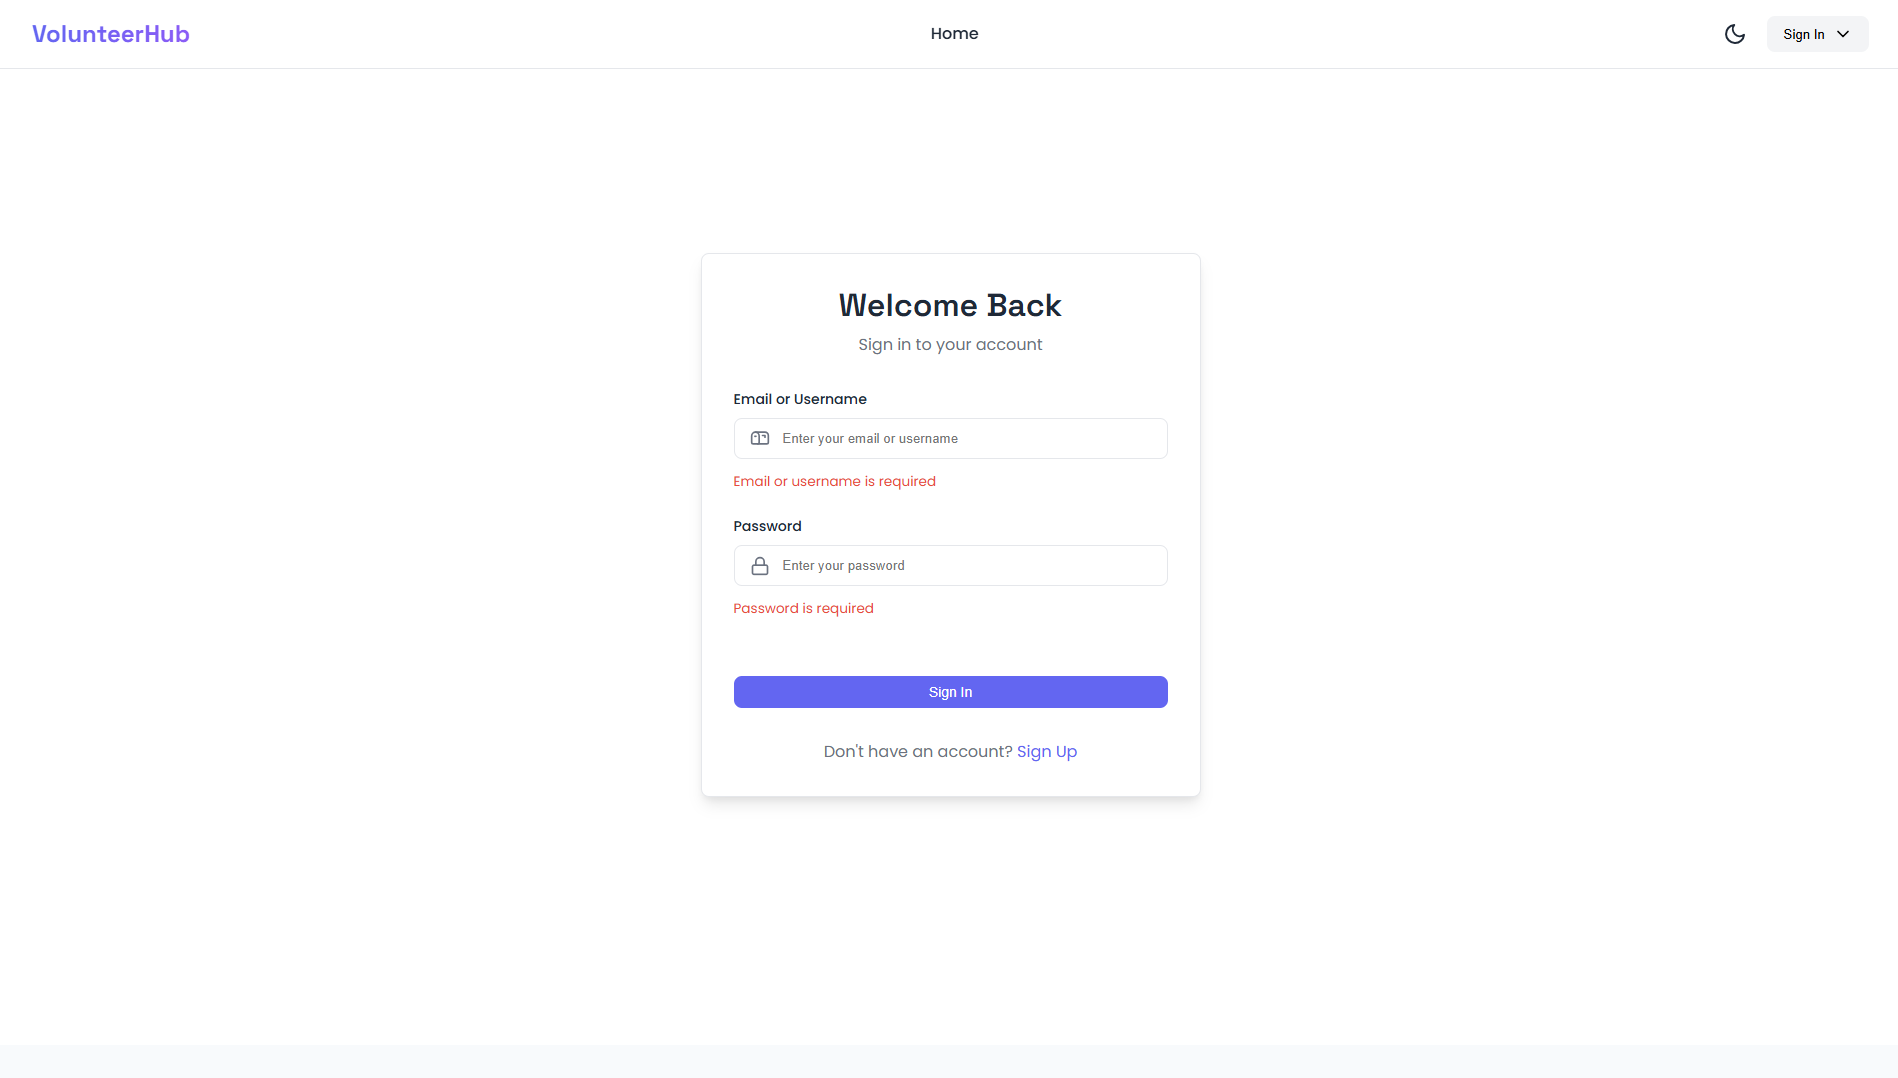
\includegraphics[width=\textwidth]{sign_in.png}
        \caption{Sign In Page}
        \label{fig:signin}
    \end{subfigure}
    \caption{User Authentication Interfaces}
    \label{fig:auth}
\end{figure}

\subsection{Admin Interfaces}
\begin{figure}[H]
    \centering
    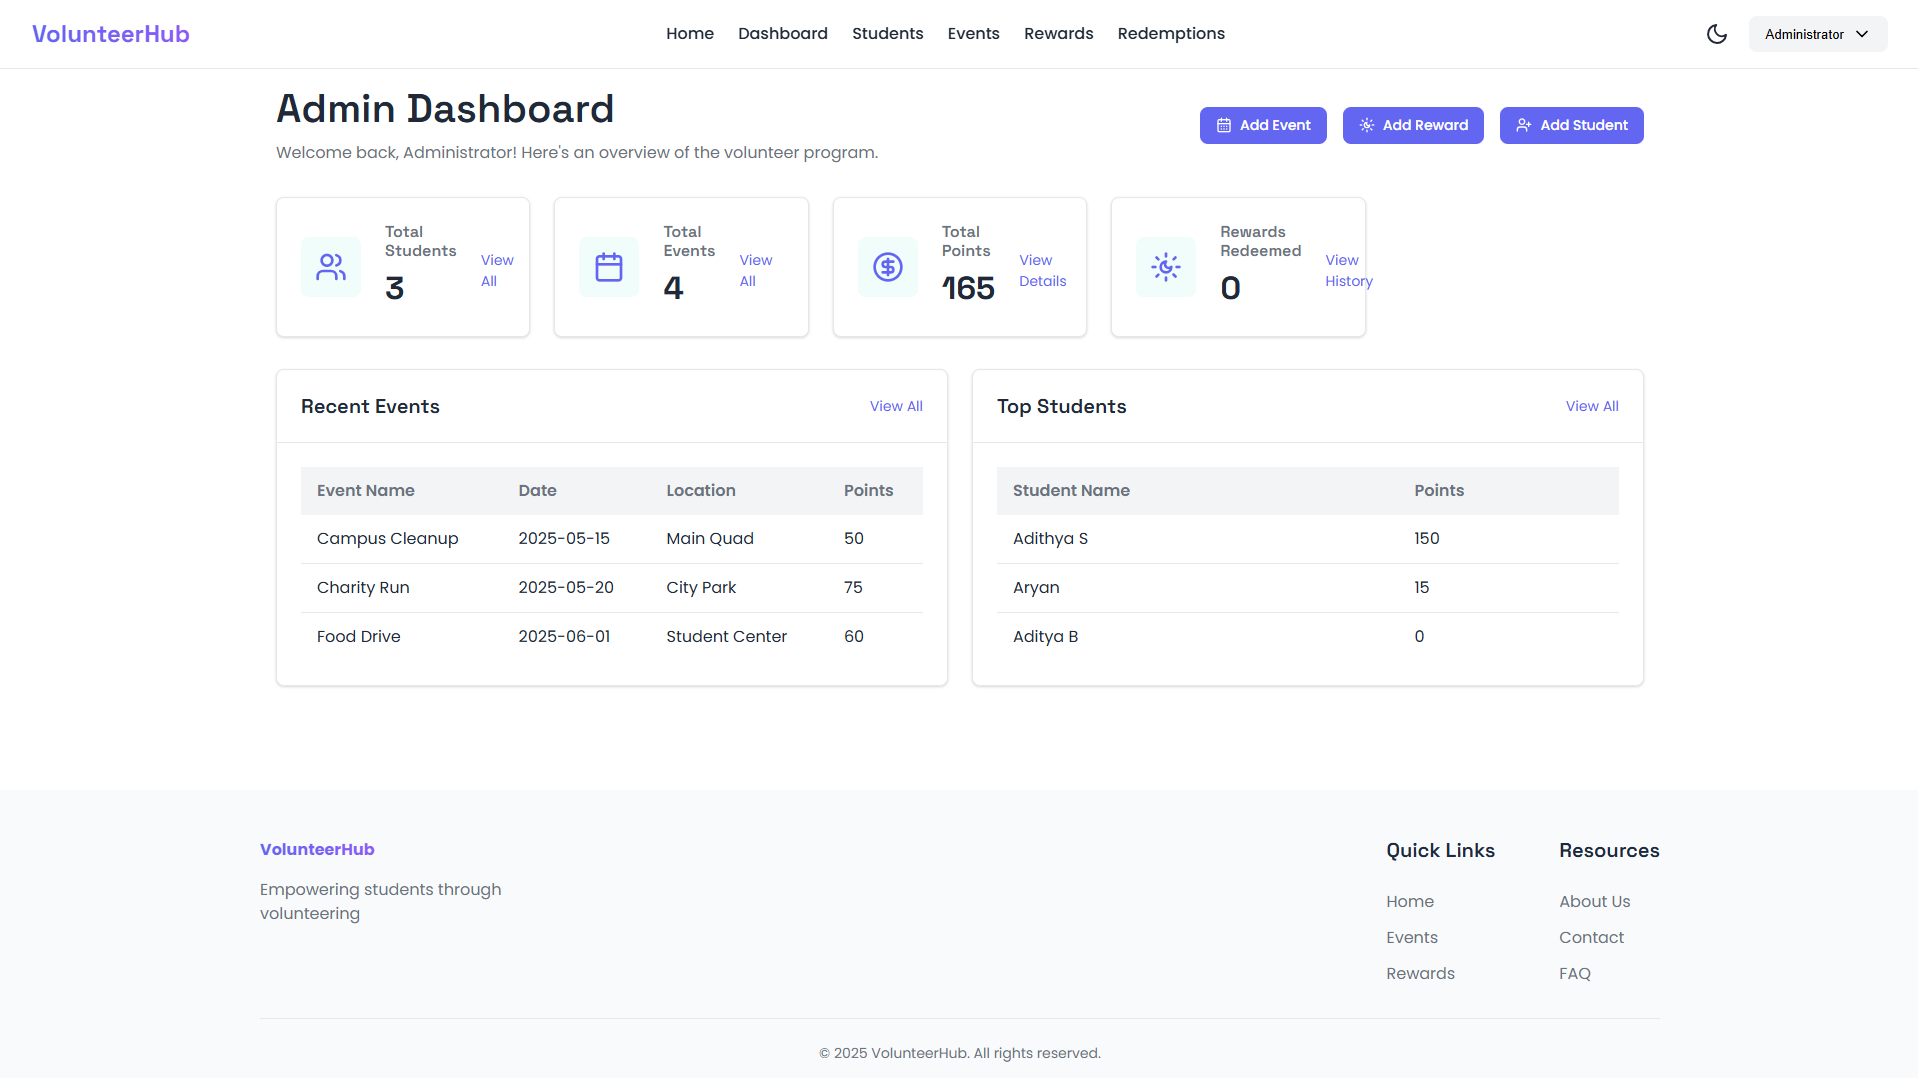
\includegraphics[width=0.8\textwidth]{admin_dashboard.png}
    \caption{Admin Dashboard}
    \label{fig:admin-dashboard}
\end{figure}

\begin{figure}[H]
    \centering
    \begin{subfigure}[b]{0.48\textwidth}
        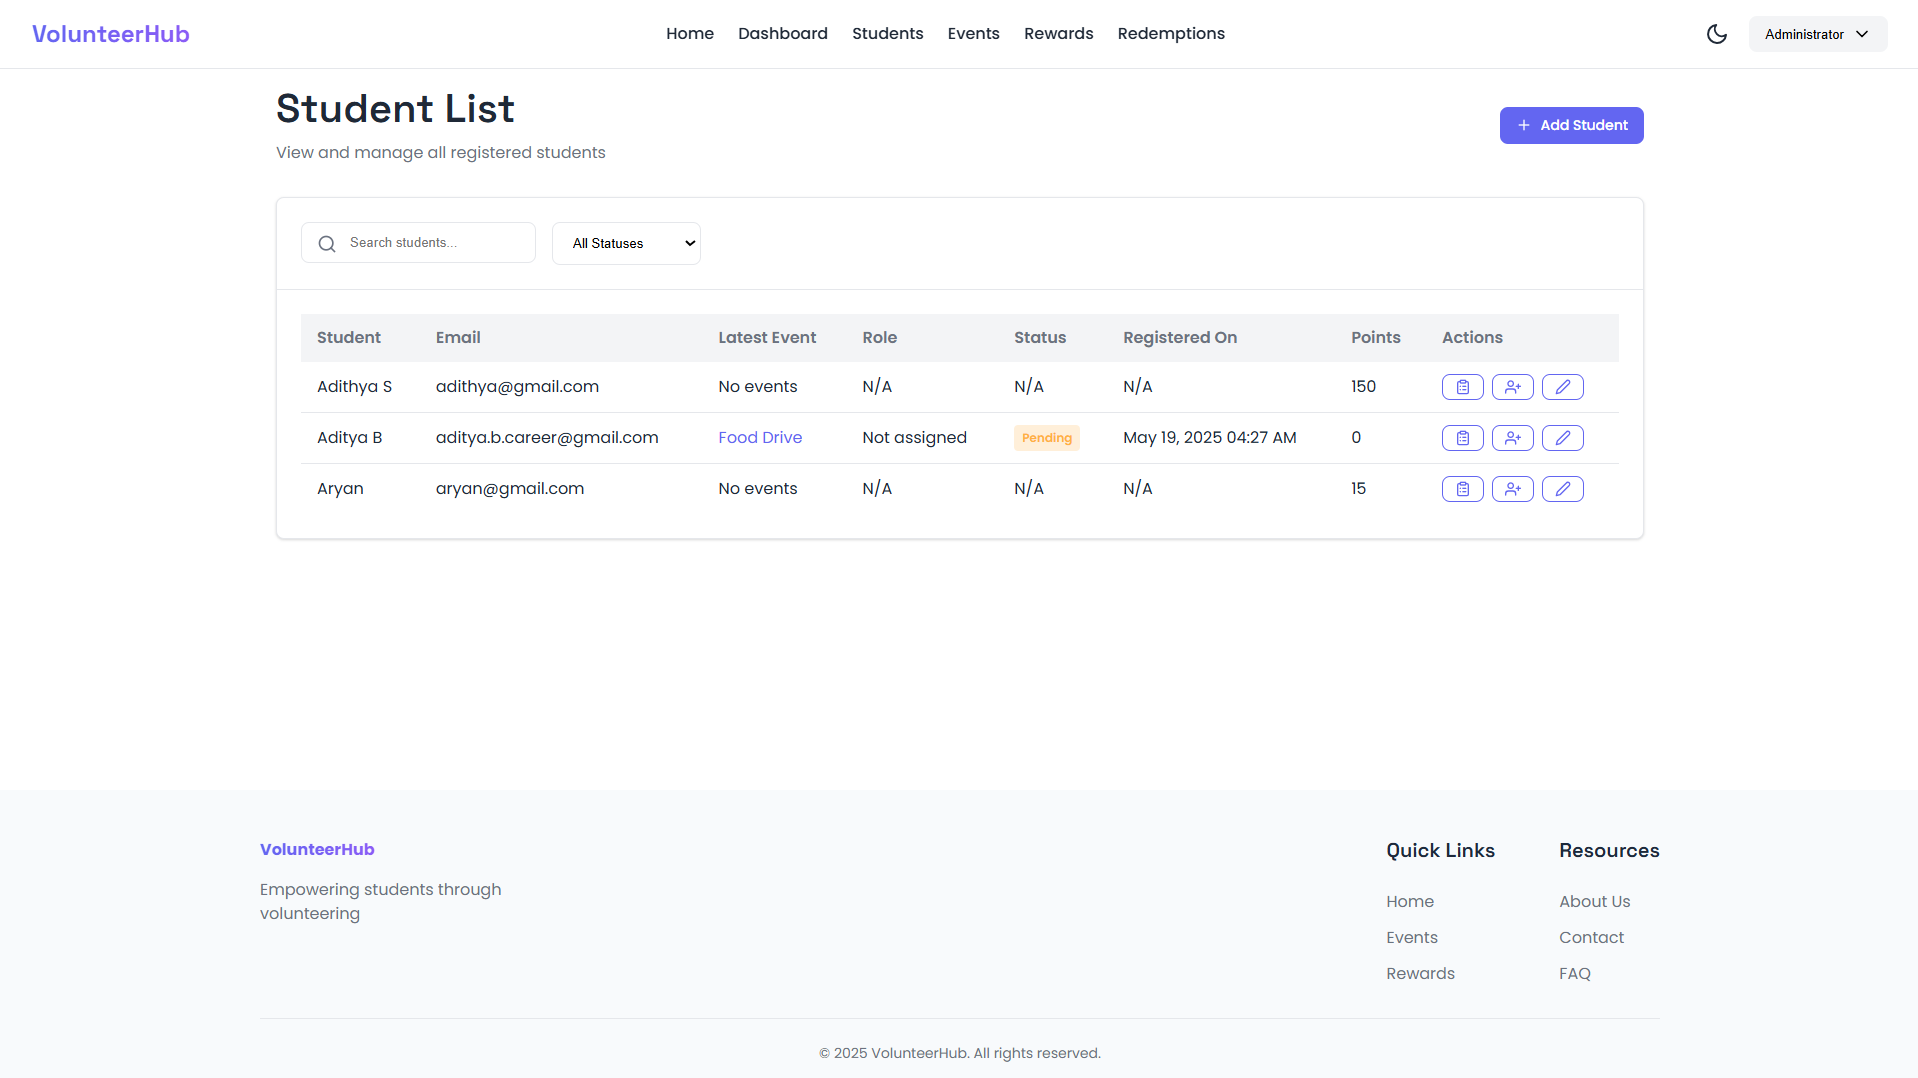
\includegraphics[width=\textwidth]{admin_student_list.png}
        \caption{Student Management}
        \label{fig:admin-students}
    \end{subfigure}
    \hfill
    \begin{subfigure}[b]{0.48\textwidth}
        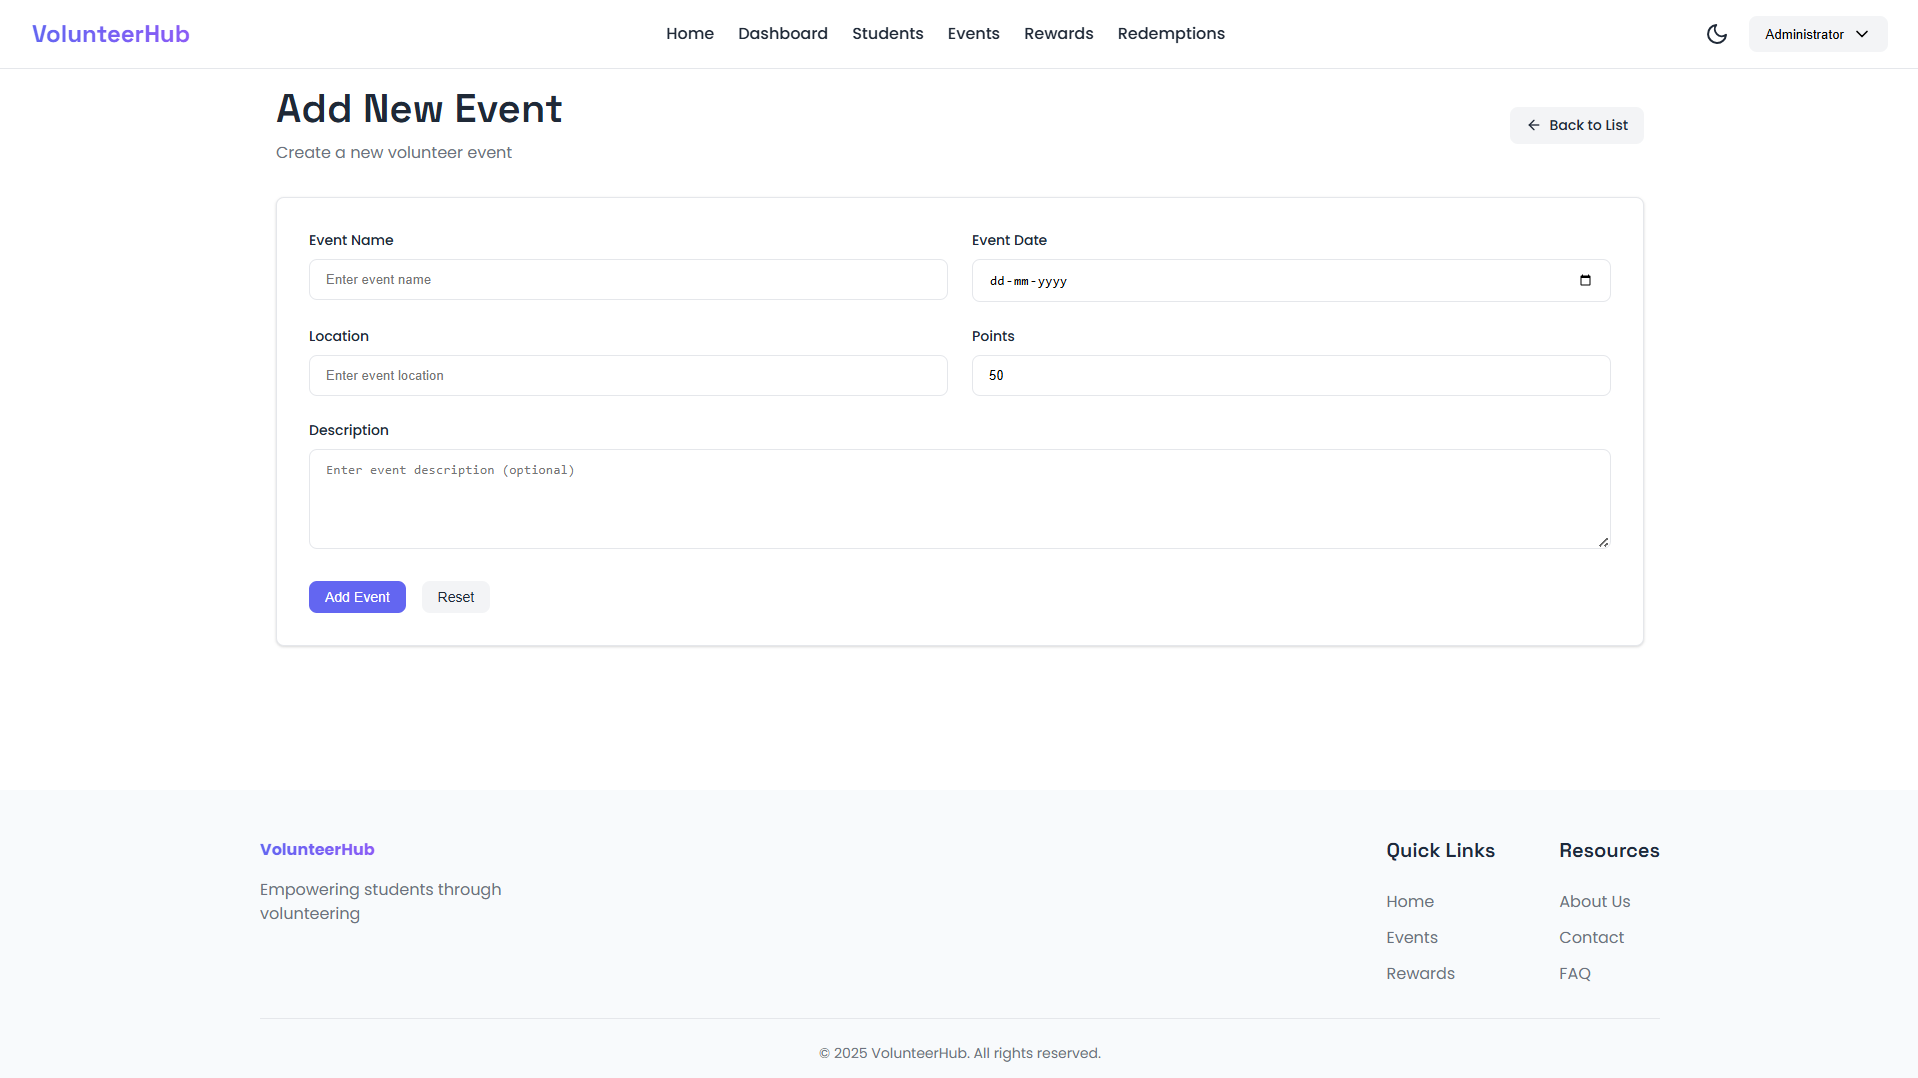
\includegraphics[width=\textwidth]{admin_add_new_event.png}
        \caption{Event Creation}
        \label{fig:admin-events}
    \end{subfigure}
    \caption{Admin Management Interfaces}
    \label{fig:admin-interfaces}
\end{figure}

\begin{figure}[H]
    \centering
    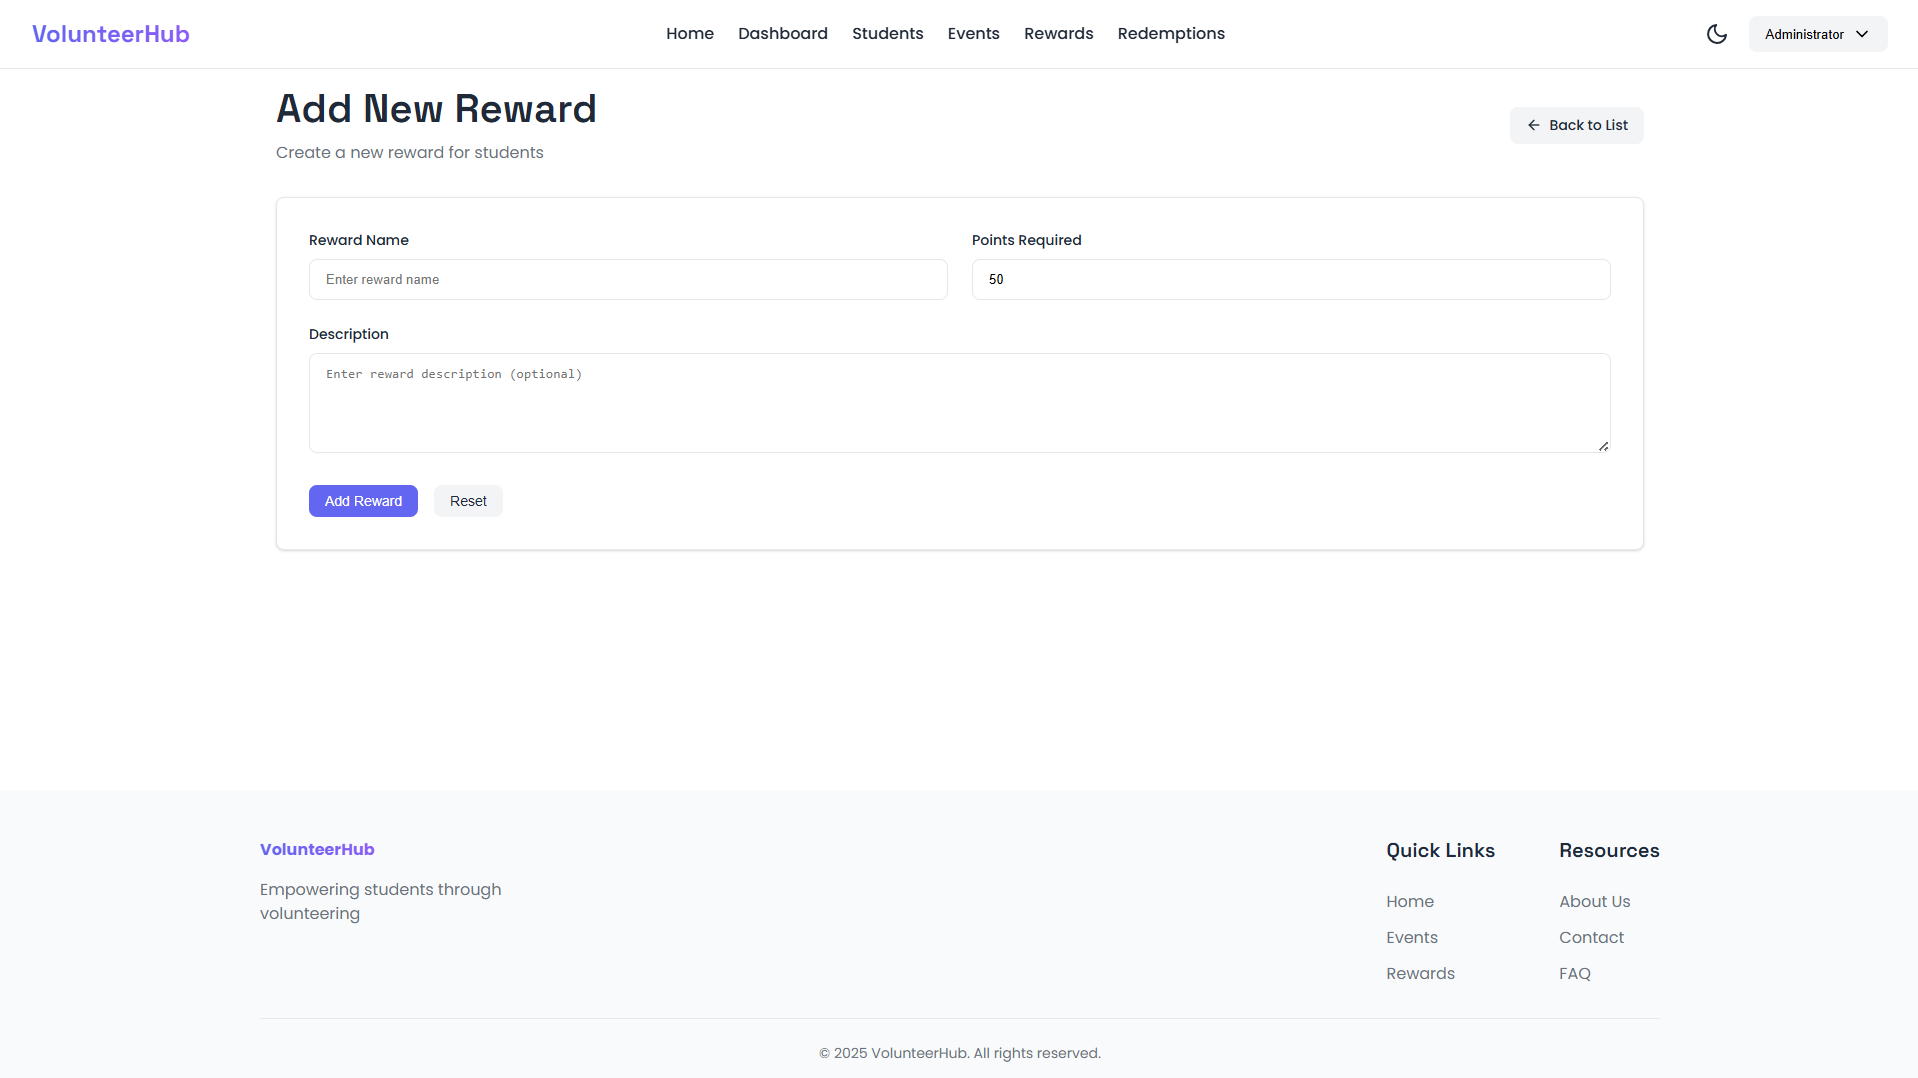
\includegraphics[width=0.8\textwidth]{admin_add_new_reward.png}
    \caption{Admin Reward Management}
    \label{fig:admin-rewards}
\end{figure}

\subsection{Student Interfaces}
\begin{figure}[H]
    \centering
    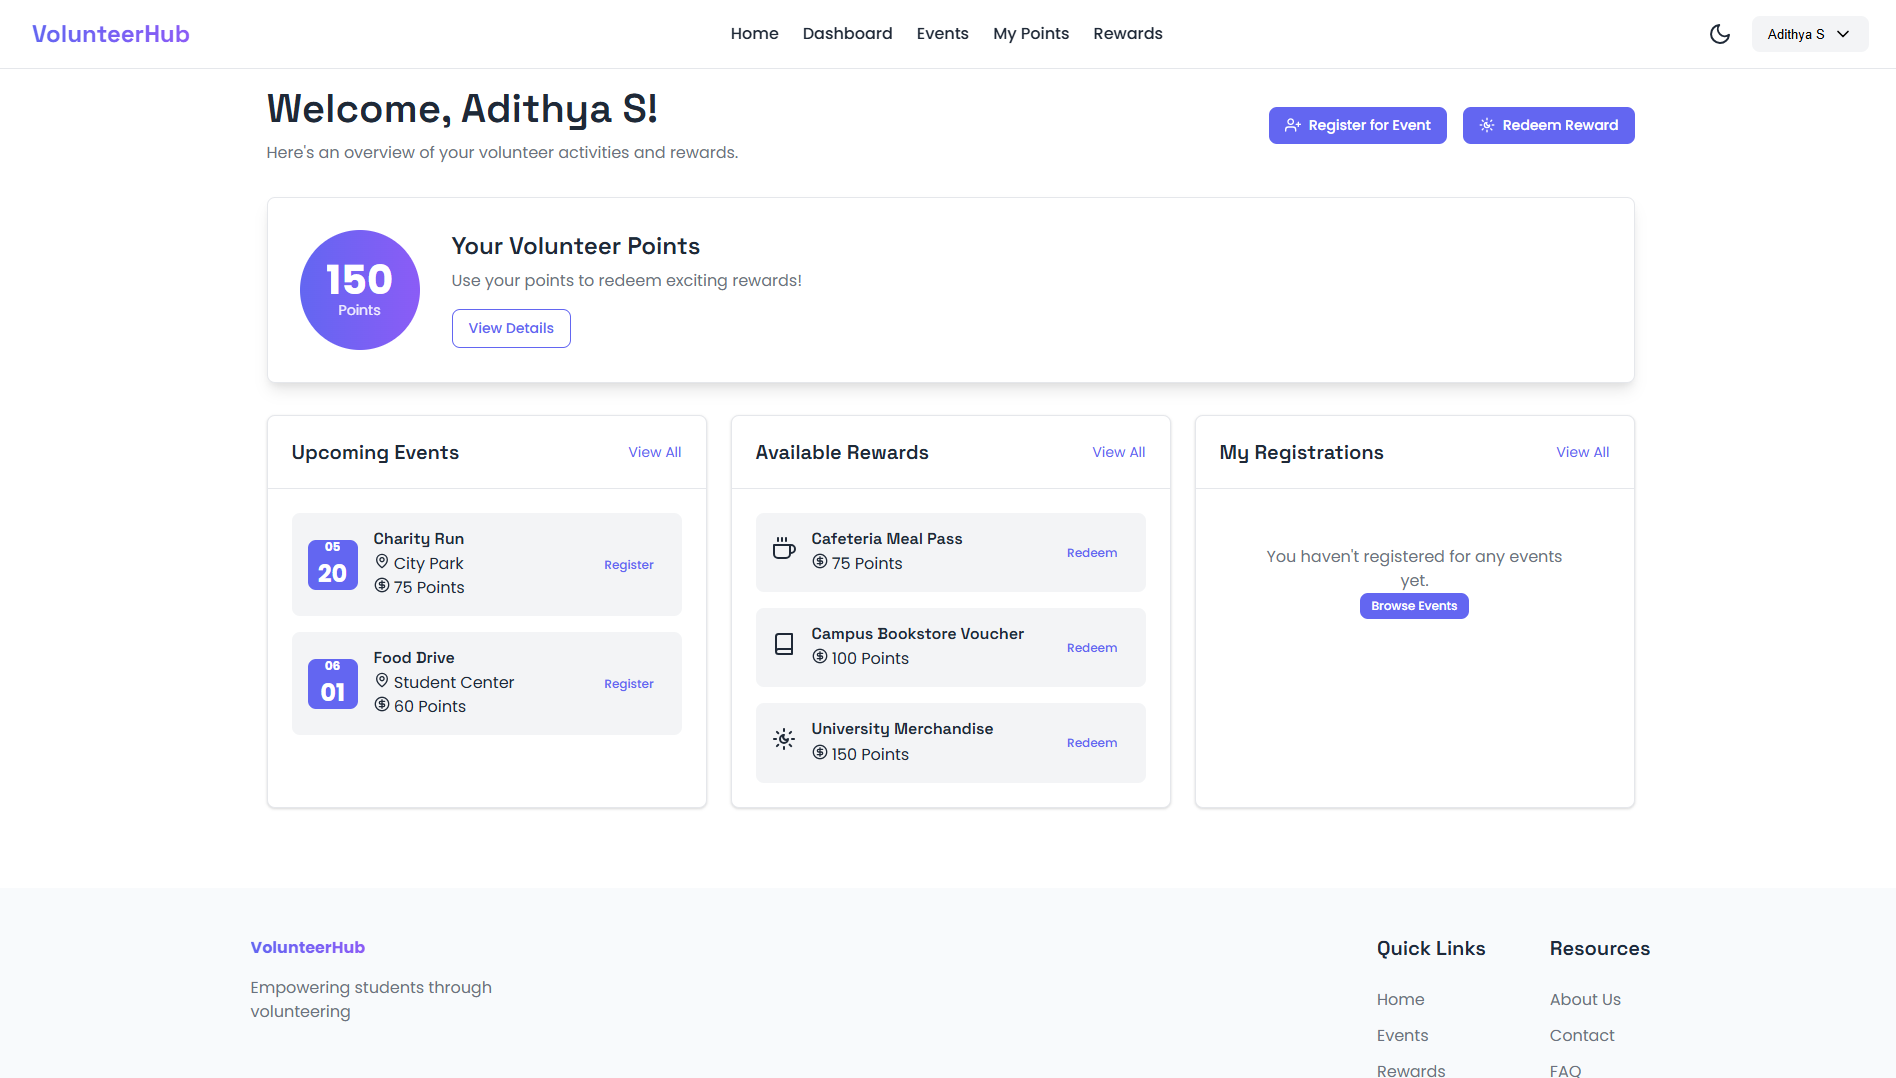
\includegraphics[width=0.8\textwidth]{Student_dashboard.png}
    \caption{Student Dashboard}
    \label{fig:student-dashboard}
\end{figure}

\begin{figure}[H]
    \centering
    \begin{subfigure}[b]{0.48\textwidth}
        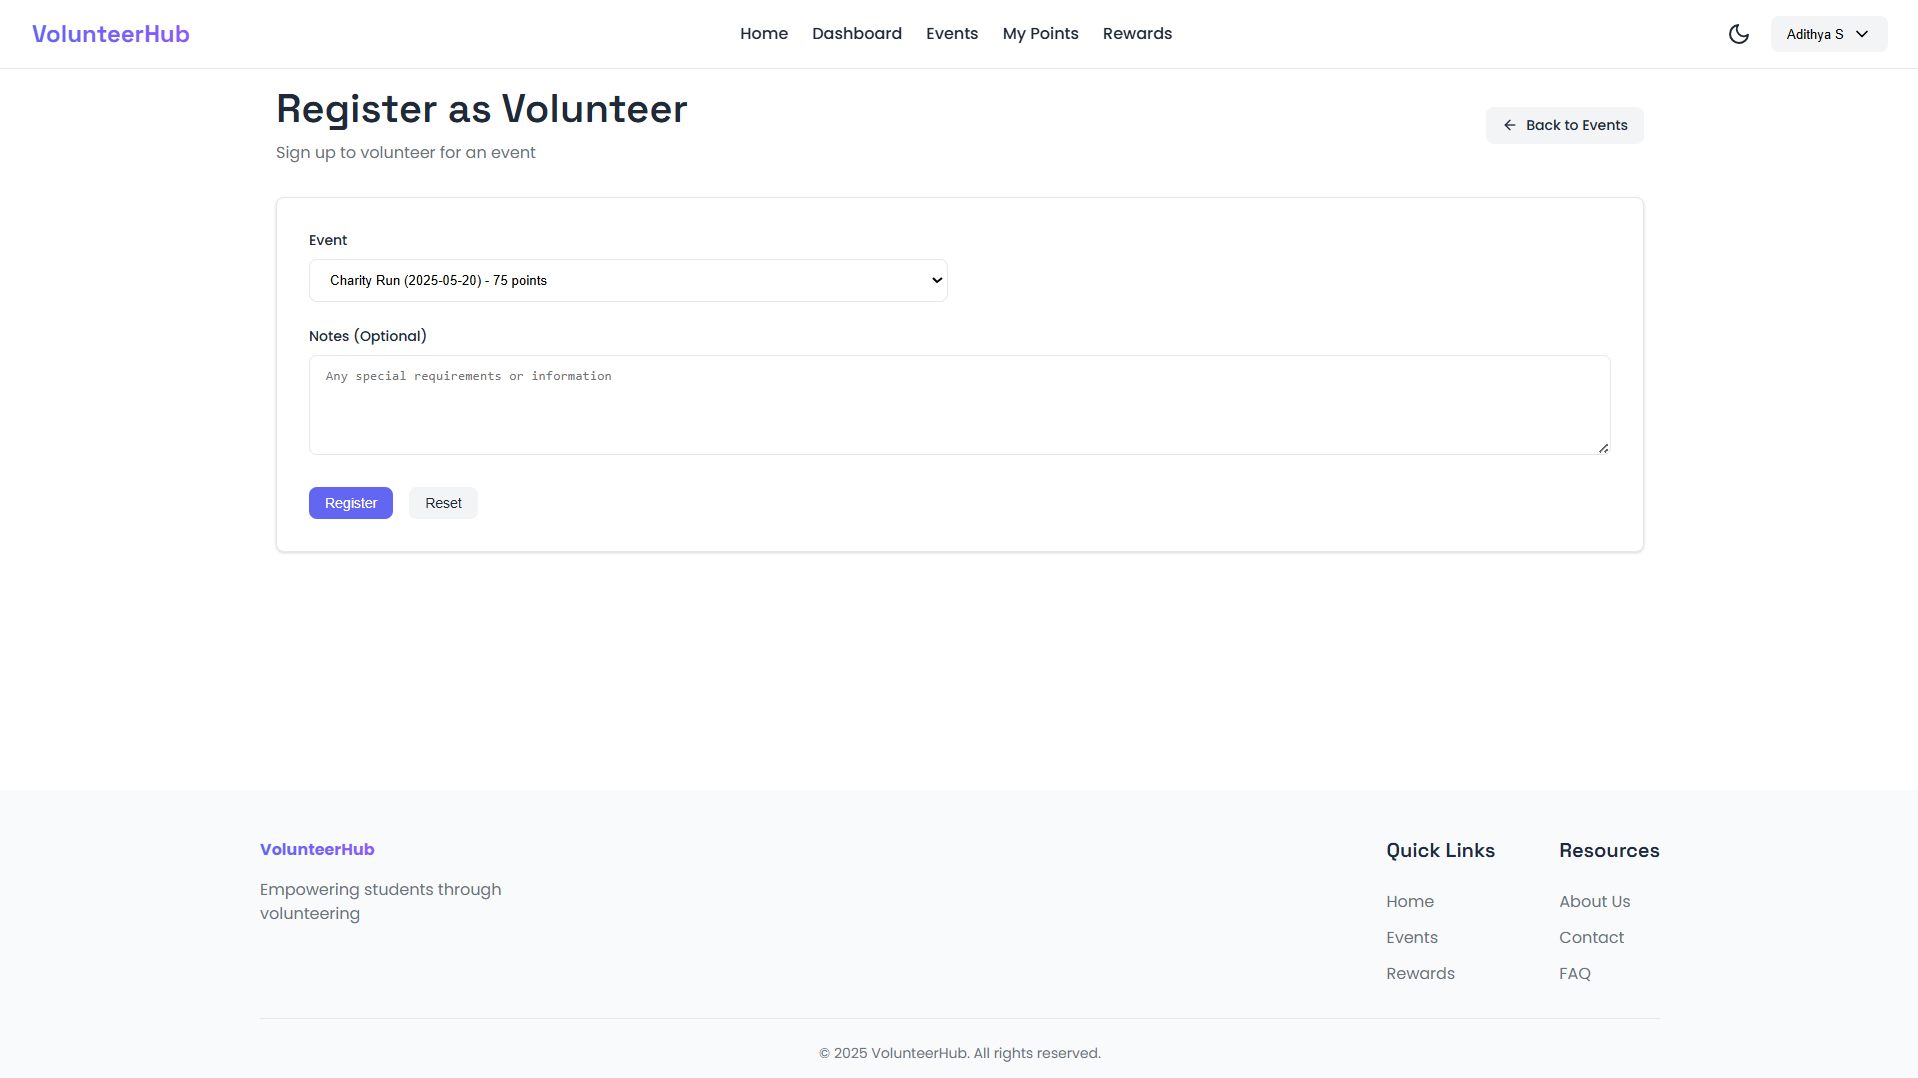
\includegraphics[width=\textwidth]{Student_Registeer.png}
        \caption{Event Registration}
        \label{fig:student-register}
    \end{subfigure}
    \hfill
    \begin{subfigure}[b]{0.48\textwidth}
        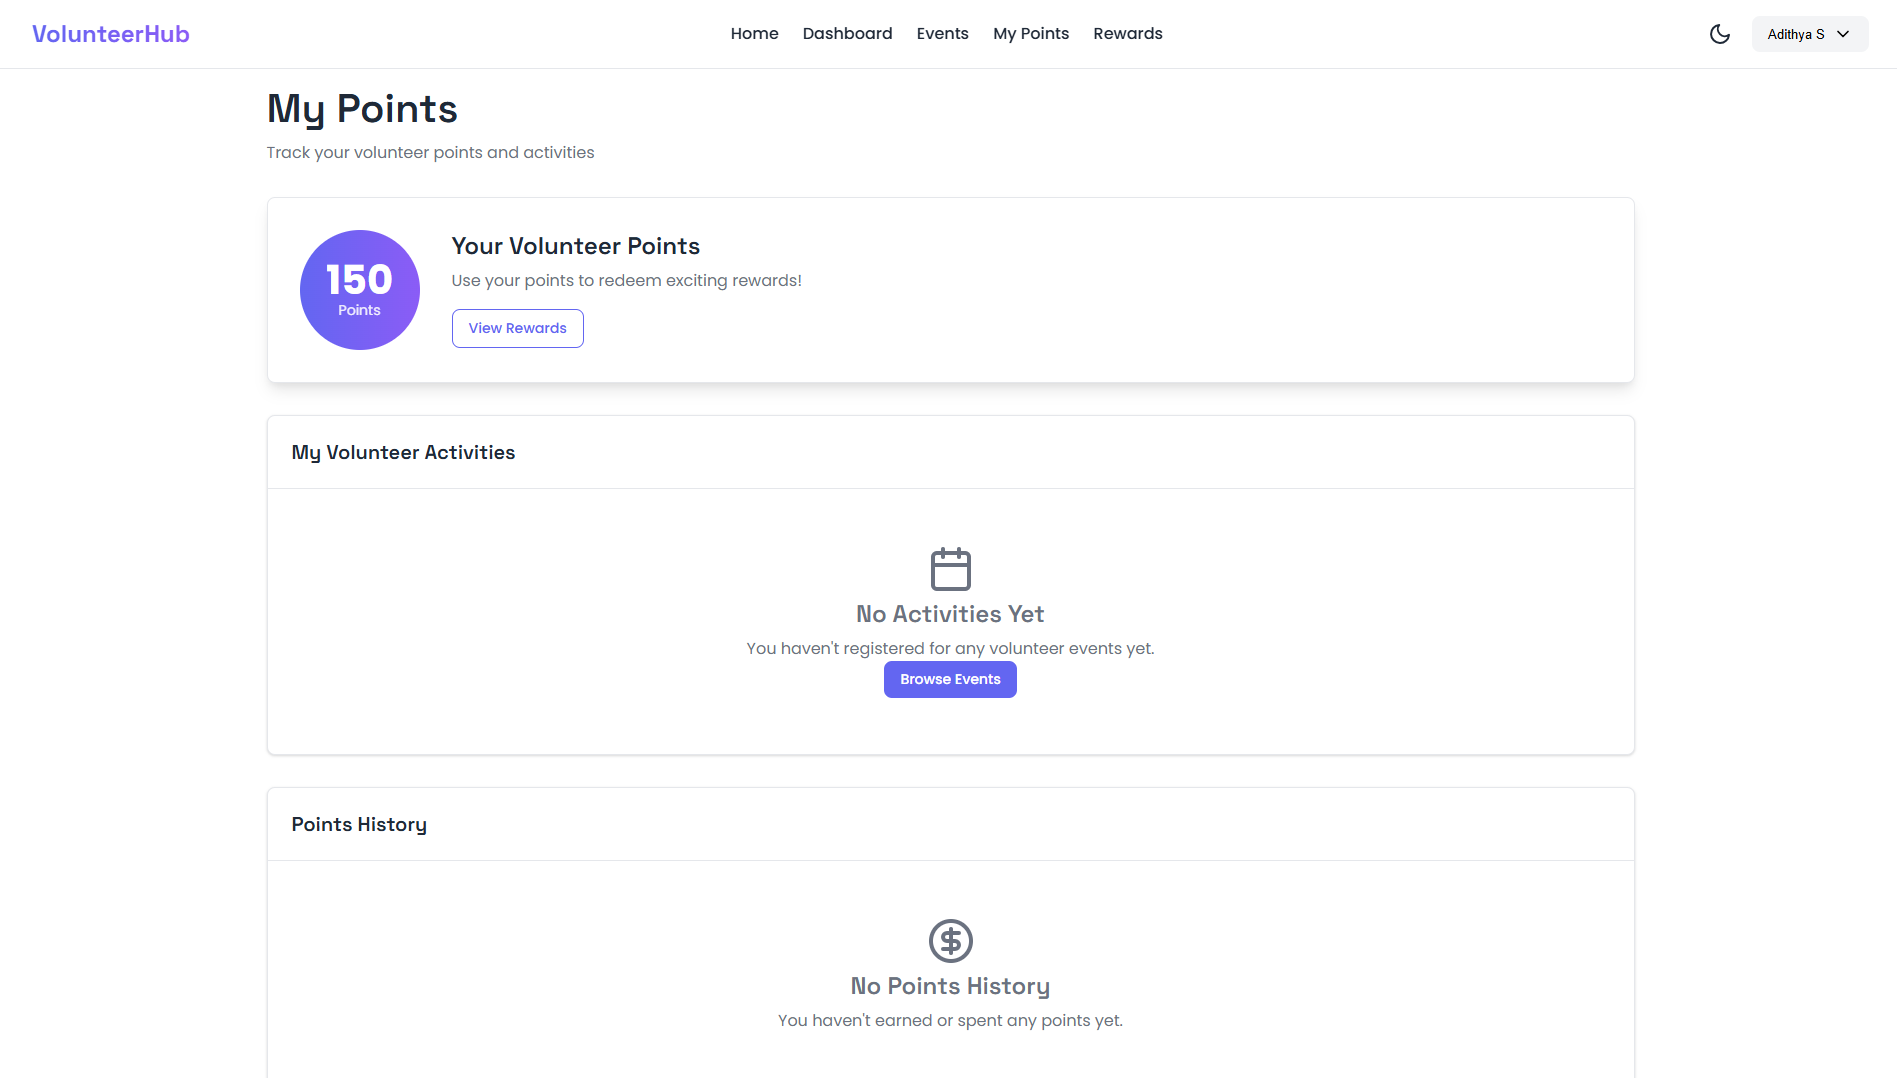
\includegraphics[width=\textwidth]{Student_My_Points.png}
        \caption{Points History}
        \label{fig:student-points}
    \end{subfigure}
    \caption{Student Activity Interfaces}
    \label{fig:student-interfaces}
\end{figure}

\begin{figure}[H]
    \centering
    \begin{subfigure}[b]{0.48\textwidth}
        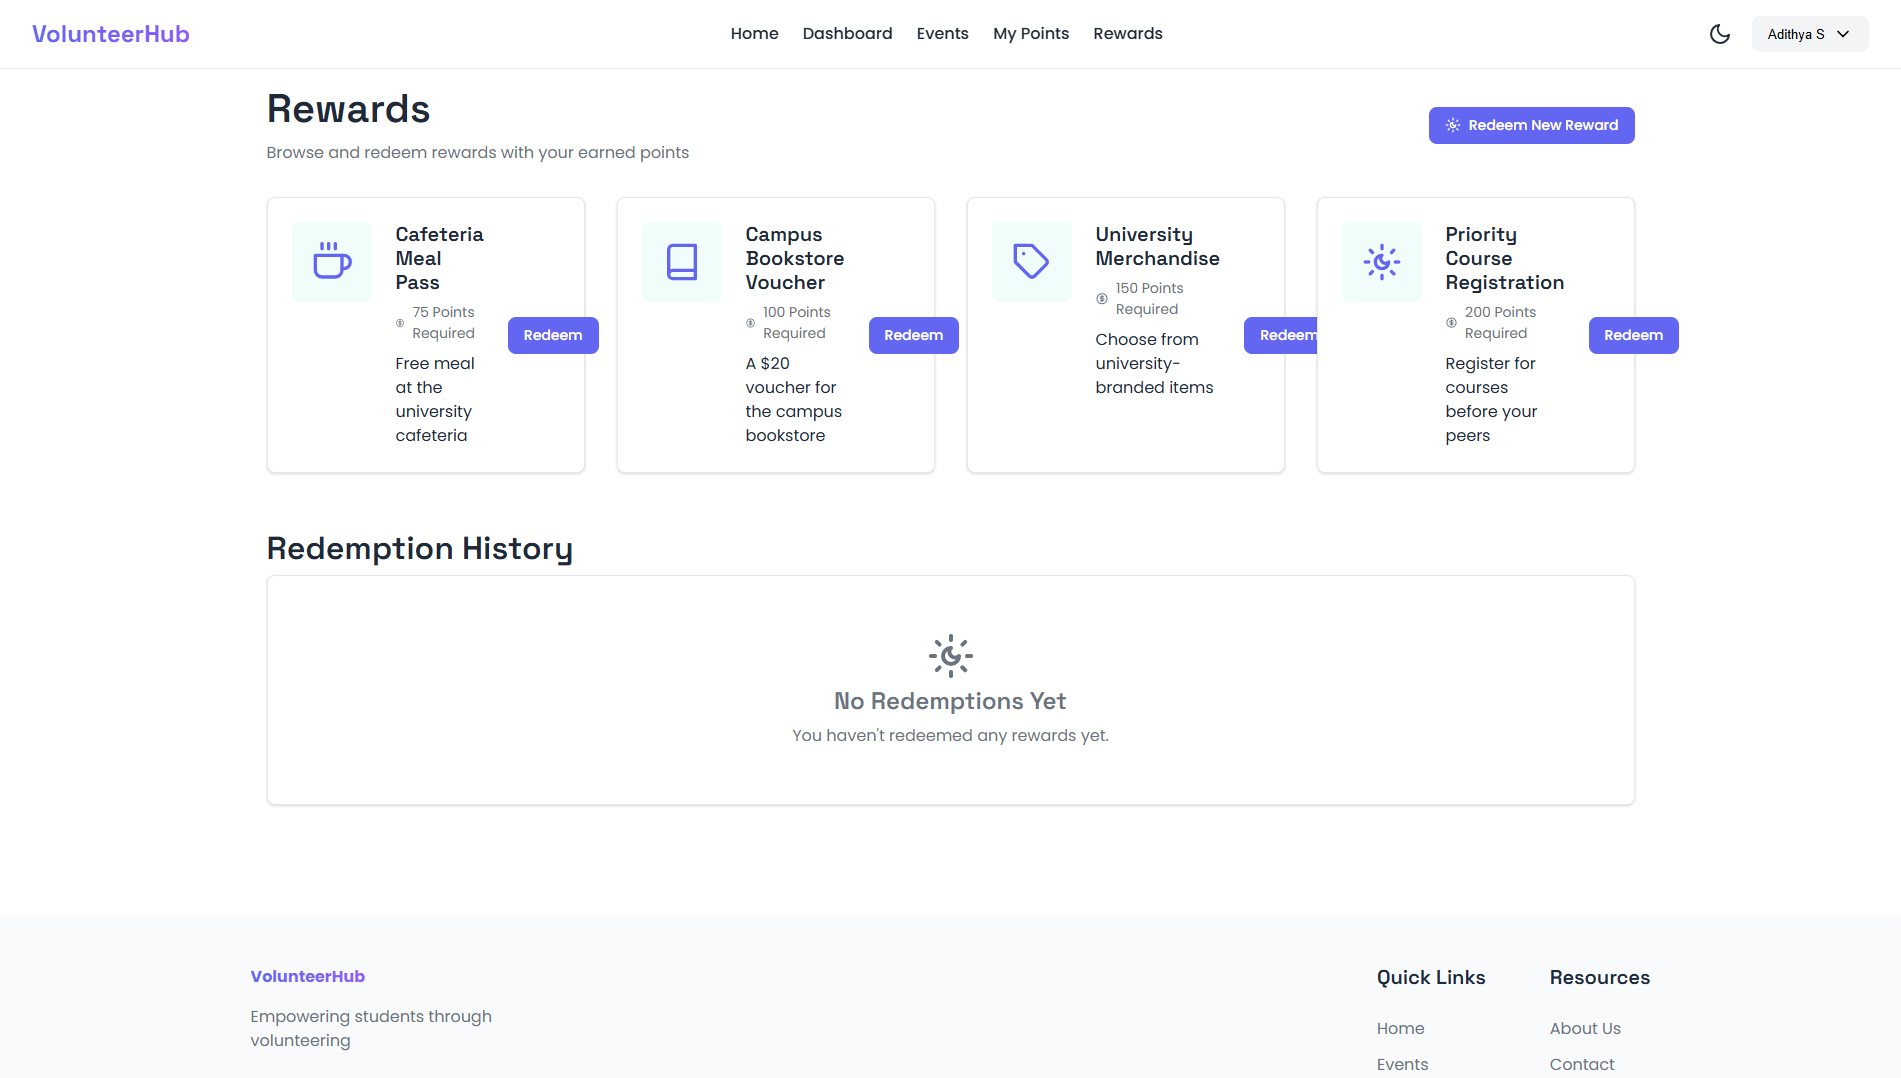
\includegraphics[width=\textwidth]{student_Redeem_rewards.png}
        \caption{Rewards Catalog}
        \label{fig:student-rewards}
    \end{subfigure}
    \hfill
    \begin{subfigure}[b]{0.48\textwidth}
        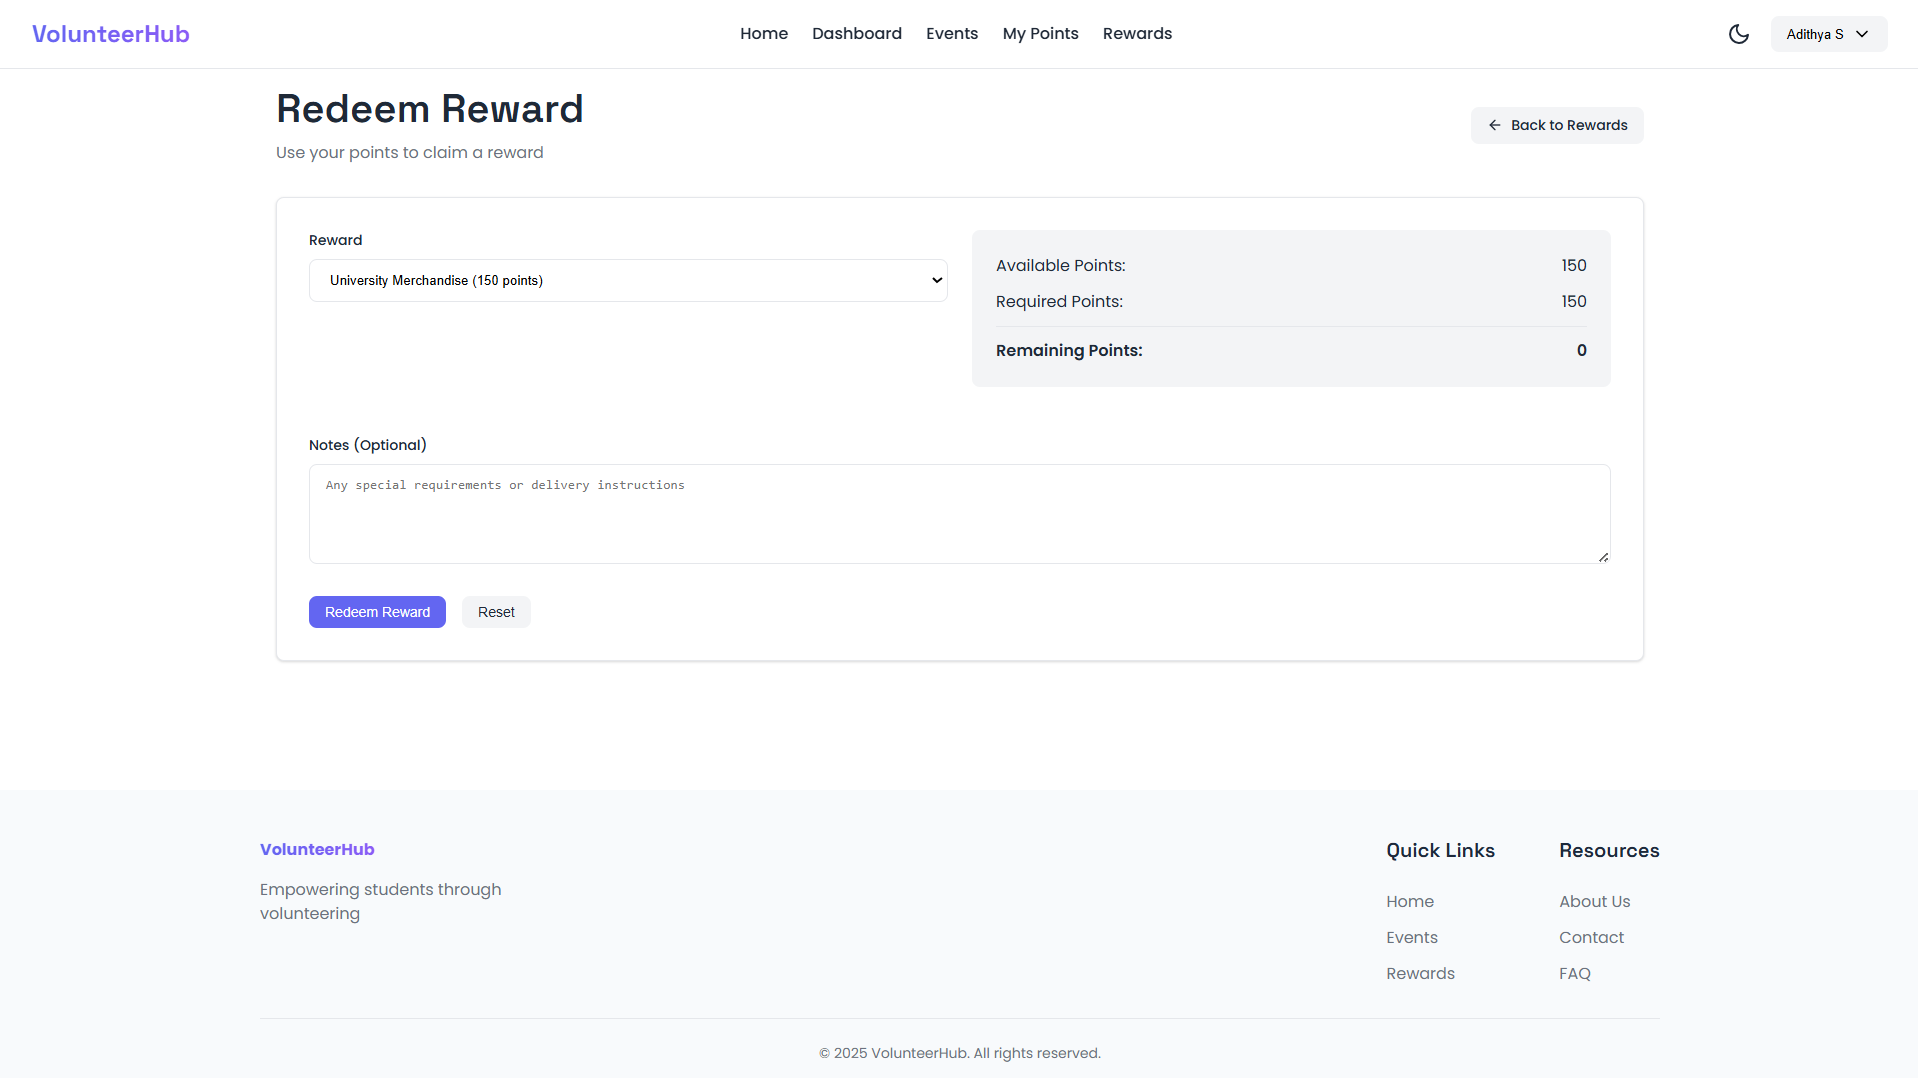
\includegraphics[width=\textwidth]{student_Redeeming_Reward.png}
        \caption{Reward Redemption}
        \label{fig:student-redeem}
    \end{subfigure}
    \caption{Reward System Interfaces}
    \label{fig:reward-interfaces}
\end{figure}

\section{Testing}

\subsection{Unit Testing}
Unit tests were created for core functionality using Python's unittest framework. Key areas tested include:

\begin{itemize}
    \item Database operations
    \item Authentication functionality
    \item Points calculation and tracking
    \item Reward redemption logic
\end{itemize}

\subsection{Integration Testing}
Integration tests verified the proper interaction between system components, focusing on:

\begin{itemize}
    \item Database and application layer integration
    \item Route handling and template rendering
    \item Session management and authentication flow
\end{itemize}

\subsection{User Interface Testing}
UI testing was conducted to ensure:

\begin{itemize}
    \item Responsive design across different screen sizes
    \item Form validation functionality
    \item Proper display of dynamic content
    \item Navigation flow between pages
\end{itemize}

\chapter{Results and Conclusion}

\section{Project Achievements}
The VolunteerHub system successfully implements:

\begin{itemize}
    \item A complete volunteer management system with dual user roles
    \item Secure authentication and authorization
    \item Comprehensive event management capabilities
    \item Points tracking and rewards redemption functionality
    \item Intuitive interfaces for both administrators and students
\end{itemize}

\section{Evaluation Against Requirements}
The implemented system meets all specified functional and non-functional requirements:

\begin{itemize}
    \item User and event management functions are fully operational
    \item The points system accurately tracks volunteer participation
    \item The rewards system enables meaningful incentivization
    \item Security measures protect user data and system integrity
    \item Performance metrics meet specified targets
\end{itemize}

\section{Key Learnings}
Through this project, we gained valuable experience and insights in:

\begin{itemize}
    \item Database design principles and normalization
    \item Web application security best practices
    \item Full-stack development with Flask
    \item User experience considerations in application design
    \item Points-based incentive system implementation
\end{itemize}

\section{Conclusion}
VolunteerHub provides an efficient solution for managing volunteer activities within educational institutions. The points-based system effectively incentivizes student participation while reducing administrative burden. The application successfully addresses the needs of both administrators and volunteers through intuitive interfaces and comprehensive functionality.

The system demonstrates how database management principles can be applied to create practical solutions that address real-world challenges in volunteer management. By centralizing volunteer data and automating key processes, VolunteerHub enhances both administrative efficiency and student engagement in volunteer activities.

\chapter{Future Enhancements}

The current implementation of VolunteerHub provides a solid foundation for volunteer management. However, several potential enhancements could further extend its capabilities:

\section{Technical Enhancements}
\begin{itemize}
    \item \textbf{Mobile Application}: Develop a dedicated mobile app for iOS and Android to enhance accessibility
    \item \textbf{API Layer}: Create a RESTful API to enable integration with other campus systems
    \item \textbf{Advanced Analytics}: Implement data visualization tools for deeper insights into volunteer participation patterns
    \item \textbf{Scalability Improvements}: Transition to a more robust database system (e.g., PostgreSQL) for larger deployments
\end{itemize}

\section{Functional Enhancements}
\begin{itemize}
    \item \textbf{Email Notifications}: Implement automated notifications for event reminders, registration confirmations, and reward redemptions
    \item \textbf{Calendar Integration}: Allow synchronization with popular calendar applications
    \item \textbf{Social Features}: Add volunteer teams, leaderboards, and social sharing capabilities
    \item \textbf{Attendance Tracking}: Implement QR code-based attendance verification for events
    \item \textbf{Volunteer Skills Database}: Create a skills inventory to better match volunteers with appropriate roles
\end{itemize}

\section{User Experience Enhancements}
\begin{itemize}
    \item \textbf{Personalized Recommendations}: Suggest events based on past participation and interests
    \item \textbf{Enhanced Profile Pages}: Allow volunteers to showcase their contributions and achievements
    \item \textbf{Volunteer Journey Map}: Visualize volunteer growth and impact over time
    \item \textbf{Customizable Dashboards}: Allow users to configure their dashboard views
\end{itemize}

\section{Administrative Enhancements}
\begin{itemize}
    \item \textbf{Report Generation}: Develop comprehensive reporting tools for administrative users
    \item \textbf{Bulk Operations}: Enable batch processing of volunteer approvals, point awards, etc.
    \item \textbf{Role-Based Permissions}: Implement more granular access controls within the admin role
    \item \textbf{Audit Logging}: Enhanced tracking of system operations for security and compliance
\end{itemize}

These potential enhancements would further strengthen VolunteerHub's value proposition and expand its utility within educational institutions and potentially beyond.


\clearpage
\phantomsection
\renewcommand{\bibname}{References} % This changes the default "Bibliography" title to "References"
\addcontentsline{toc}{chapter}{References}

\begin{thebibliography}{9}
    \bibitem{ieee1} S. Sharma and M. Dhiman, "A Comprehensive Review of Volunteer Management Systems: Challenges and Future Directions," \textit{IEEE Access}, vol. 9, pp. 127640-127653, 2021.
    
    \bibitem{ieee2} P. Kumar, R. Singh, and A. Tripathi, "BlockVMS: Blockchain-Based Volunteer Management System for Transparent Community Service," \textit{IEEE Transactions on Engineering Management}, vol. 70, no. 5, pp. 1766-1780, 2023.
    
    \bibitem{acm1} J. Wang, S. Li, and Y. Chen, "Gamification in Volunteer Engagement: A Systematic Review," in \textit{Proceedings of the 2022 ACM Conference on Human Factors in Computing Systems (CHI '22)}, pp. 1-15, 2022.
    
    \bibitem{acm2} M. Brown and K. Davis, "PointsWork: A Points-Based Incentive System for Student Volunteer Management," in \textit{Proceedings of the 2021 ACM Conference on Computer Supported Cooperative Work and Social Computing}, pp. 267-278, 2021.

    \bibitem{springer1} R. González-Pérez and A. García-Holgado, "Digital Platform for Volunteer Management: A Case Study in Higher Education," in \textit{Advances in Human-Computer Interaction: Proceedings of HCI International 2022}, Springer, Cham, pp. 189-204, 2022.
    
    \bibitem{flask} Flask Documentation, \url{https://flask.palletsprojects.com/}
    
    \bibitem{sqlite} SQLite Documentation, \url{https://www.sqlite.org/docs.html}
    
    \bibitem{python} Python Documentation, \url{https://docs.python.org/3/}
    
    \bibitem{db_design} C.J. Date, "An Introduction to Database Systems," 8th Edition, Pearson, 2022.
    
    \bibitem{web_dev} Miguel Grinberg, "Flask Web Development: Developing Web Applications with Python," 2nd Edition, O'Reilly Media, 2018.
\end{thebibliography}

% Appendices (Optional)
\appendix

\chapter{SQL Schema}
\begin{lstlisting}[caption={Complete Database Schema}, label={lst:full-schema}]
CREATE TABLE students (
    id INTEGER PRIMARY KEY AUTOINCREMENT,
    name TEXT NOT NULL,
    email TEXT UNIQUE NOT NULL,
    password TEXT NOT NULL,
    phone TEXT,
    created_at TIMESTAMP
);

CREATE TABLE events (
    id INTEGER PRIMARY KEY AUTOINCREMENT,
    name TEXT NOT NULL,
    date TEXT NOT NULL,
    location TEXT NOT NULL,
    points INTEGER NOT NULL,
    description TEXT,
    created_at TIMESTAMP
);

CREATE TABLE registrations (
    id INTEGER PRIMARY KEY AUTOINCREMENT,
    student_id INTEGER NOT NULL,
    event_id INTEGER NOT NULL,
    role_assigned TEXT,
    status TEXT DEFAULT 'Pending',
    created_at TIMESTAMP,
    FOREIGN KEY (student_id) REFERENCES students (id),
    FOREIGN KEY (event_id) REFERENCES events (id)
);

CREATE TABLE points (
    id INTEGER PRIMARY KEY AUTOINCREMENT,
    student_id INTEGER UNIQUE NOT NULL,
    points INTEGER DEFAULT 0,
    created_at TIMESTAMP,
    updated_at TIMESTAMP,
    FOREIGN KEY (student_id) REFERENCES students (id)
);

CREATE TABLE rewards (
    id INTEGER PRIMARY KEY AUTOINCREMENT,
    name TEXT NOT NULL,
    points_required INTEGER NOT NULL,
    description TEXT,
    created_at TIMESTAMP
);

CREATE TABLE redemptions (
    id INTEGER PRIMARY KEY AUTOINCREMENT,
    student_id INTEGER NOT NULL,
    reward_id INTEGER NOT NULL,
    points_used INTEGER NOT NULL,
    notes TEXT,
    created_at TIMESTAMP,
    FOREIGN KEY (student_id) REFERENCES students (id),
    FOREIGN KEY (reward_id) REFERENCES rewards (id)
);

CREATE TABLE points_history (
    id INTEGER PRIMARY KEY AUTOINCREMENT,
    student_id INTEGER NOT NULL,
    points_change INTEGER NOT NULL,
    reason TEXT NOT NULL,
    created_at TIMESTAMP,
    FOREIGN KEY (student_id) REFERENCES students (id)
);
\end{lstlisting}

\chapter{Project Timeline}
\begin{table}[H]
    \centering
    \begin{tabular}{|l|l|p{8cm}|}
        \hline
        \textbf{Day} & \textbf{Phase} & \textbf{Tasks Completed} \\
        \hline
        1-2 & Requirements Analysis & Problem definition, user stories, requirements specification \\
        \hline
        3-4 & Design & Database design, architecture planning, UI wireframing \\
        \hline
        5-7 & Implementation (Core) & Database setup, authentication, basic CRUD operations \\
        \hline
        8-10 & Implementation (Features) & Points system, rewards system, admin functions \\
        \hline
        11-12 & Testing & Unit tests, integration tests, UI testing \\
        \hline
        13-14 & Refinement & Bug fixes, performance optimization, UI improvements \\
        \hline
        15 & Documentation & Final documentation, user guides \\
        \hline
    \end{tabular}
    \caption{Project Development Timeline}
    \label{tab:timeline}
\end{table}

\end{document}